\documentclass[12pt,fleqn]{book}
\usepackage{amsmath} %utk masuk begin{align}
\usepackage{amsxtra}%supaya \eqref
\usepackage{amsopn}%supaya dapat declare benda baru \citep
\usepackage{amsbsy}
\usepackage{amstext}
\usepackage{amsfonts}
\usepackage{amssymb}
\usepackage{amsthm}
\usepackage{shadow}% kotak shadow
\usepackage{chaptengah}
\usepackage{curves}
\usepackage{graphicx}
\usepackage{color}%masukan color
\usepackage{maple2e}
%\usepackage{flafter}
\usepackage{afterpage}
%\usepackage{tocloft}
\usepackage{XTocinc}% utk center contents, masuk chapter, topic dan page number
%  bila masuk ini jadi bold tex
%\usepackage[bottom=0.5in]{geometry}
\usepackage{lipsum}
\usepackage{imakeidx}
\makeindex
%-----------------------
\usepackage{titletoc} 
\makeatletter
\renewcommand*{\@dotsep}{999}% untuk buang dotted line besar nombor spt spt 999
\makeatother
\newtheorem{ts}{Task}
%------------------------
%--------%---
%
%\titlecontents{section}[1.5em]
 % {\bfseries}
  %{\contentslabel{2em}}
  %{\hspace*{-2.3em}}
  %{\titlerule*[1pc]{.}\contentspage} 
\usepackage{natbib}
%\makeindex
 \citestyle{mn}%\documentclass[11pt,fleqn]{report}

%\usepackage{mn}
\theoremstyle{plain}
\newtheorem{thm}{Theorem}[section]
\newtheorem{cor}[thm]{Corollary}
%\newtheorem{lem}[thm]{Lemma}
\newtheorem{prop}[thm]{Proposition}
%
%\theoremstyle{Example}
\newtheorem{exl}{Example}[section]
%
\newcommand{\sn}{\textbf{Solution}}
\theoremstyle{plain}
%\newtheorem{thm}{Theorem}[section]
%\newtheorem{cor}[thm]{Corollary}
%\newtheorem{lem}[thm]{Lemma}
%\newtheorem{prop}[thm]{Proposition}
%
\theoremstyle{Example}
%\newtheorem{exl}{Example}%section]
\theoremstyle{Question}
\newtheorem{qs}{Question}
\theoremstyle{Task}
%\newtheorem{ts}{Task}
\theoremstyle{Solution Task}
\newtheorem{sots}{Answer}
\theoremstyle{Exercise}
\newtheorem{ex}{Exercise}%section]

%
\theoremstyle{definition}
\newtheorem{defn}{Definition}[section]
%
\theoremstyle{solution}
\newtheorem{so}{Solution}
%\theoremstyle{}
%\newtheorem{qs}{}[]

\theoremstyle{remark}
\newtheorem{rem}{Remark}[section]
\newcommand{\Lim}{\mathop{\mathrm{\lim}}\limits}

%


%\theoremstyle{Problem Solving}
\newtheorem{prob}{Problem Solving}[chapter]
%
%\theoremstyle{Solution to Problem}
\newtheorem{sop}{Solution to Problem Solving}[chapter]
%
%\theoremstyle{Solution}
%\newtheorem{so}{Solution}[section]
%---------
%
%\newcommand{\Lim}{\mathop{\mathrm{\lim}}\limits}
\newcommand{\A}{\mathop{\mathrm{A}}\limits}
\newcommand{\B}{\mathop{\mathrm{B}}\limits}
\newcommand{\C}{\mathop{\mathrm{C}}\limits}
\newcommand{\D}{\mathop{\mathrm{D}}\limits}
\newcommand{\E}{\mathop{\mathrm{E}}\limits}
\newcommand{\ra}{\mathop{\longrightarrow\longrightarrow}\limits}

%\theoremstyle{Question}
%\newtheorem{qs}{Question}
%------------------
%\theoremstyle{definition}
%\newtheorem{defn}{Definition}[section]
%
%\theoremstyle{Key Term}
\newtheorem{term}{Key Term}[section]

%\theoremstyle{remark}
%\newtheorem{rem}{Remark}[section]
%
%\newtheorem{exl}{Example}[section]
%\newtheorem{so}{Solution}[section]
%\newtheorem{la}{\mathfrak{L}\{\}}[section]
\newcommand{\lap}{\mathop{\mathfrak{L}}\limits}
%--------------------
\newcommand{\mut}{\mathop{\mathfrak{U}}\limits}
\newcommand{\lapi}{\mathop{\mathfrak{L}^{-1}}\limits}
%---------

\oddsidemargin 0.6cm \evensidemargin 0in
%\addtolength{\hoffset}{3.0cm}
\marginparwidth 15pt \marginparsep 7pt
\topmargin 1.5cm %asal1.5
\headsep 1.0cm %asal 1.1
\addtolength{\voffset}{-2.6cm}%adjust 1.25m page no. dari tepi atas
\textheight 22.0cm \textwidth 16.0cm %asal 25.2
%\voffset=0.25cm
\headheight=13pt
\setcounter{chapter}{0}
\pagestyle{headings}
%\pagestyle{plain}
%\setcounter{page}{8}
\begin{document}
\setcounter{tocdepth}{4}    %How many levels to include in TOC
\addtocontents{toc}{\protect\sloppy}    %Keeps long chapters within page # margins
\pagenumbering{roman}
\tableofcontents
\pagenumbering{arabic}
\setcounter{chapter}{2}
\chapter{Non homogeneous BVP}
\section{Heat Equation}
\begin{center}------------------------------------------------------------------------------\end{center}
Suppose that $r$ is positive constant. Solve 
\begin{align*}
ku_{xx}+r&=u_t,\,\,0<x<1,\,t>0\\
s.t\,\,\,&\\
u(0,t)=0,\,\,u(L,t)&=u_0,\,t>0\\
u(x,o)&=f(x),\,0<x<1
\end{align*}
\begin{center}-------------------------------------------------------------------------------------\end{center}
\shabox{General Solution}
\begin{align*}
u(x,t)&=-\frac{r}{2k}x^2+\left(\frac{r}{2k}+u_0\right)x+\sum_{n=1^\infty}\,A_n\,e^{-kn^2\pi^2t}\sin\,n\pi x
\end{align*}
where 
\begin{equation}
A_n=2\int_0^1\left[f(x)+\frac{r}{2k}x^2-\left(\frac{r}{2k}+u_0\right)\right]\sin\,n\pi x\,dx\label{an}
\end{equation}
\section{Exercise 12.6}
\begin{prob}
\shabox{Q1}Use Method1
\end{prob}
Solve the equation 
\begin{equation}
ku_{tt}=u_t,\,0<x<1,\,t>0\label{pde1}
\end{equation}
 subject to
\begin{align*}
u(0,t)=100,\,\,u(1,t)=100\\
u(x,0)=0
\end{align*}
%where 
%%\begin{equation*}
%A_n=2\int_0^1\left[f(x)+\frac{r}{2k}x^2-\left(\frac{r}{2k}+u_0\right)\right]\sin\,n\pi x\,dx
%\end{equation*}
\begin{center}-------------------------------------\end{center}
\begin{sop}
\end{sop}
By changing the dependent variable $u$ to a new dependent variable $\nu$ by substitution 
\begin{equation}
u(x,t)=\nu(x,t)+\psi(x)\label{v1}
\end{equation}
Here $r=0$, $f(x)=0$.
Substitute \eqref{v1} into \eqref{pde1} gives
\begin{equation}
k\nu_{xx}+k\psi_{xx}=\nu_t\label{pde2}
\end{equation}
Problem A:
\begin{align}
k\psi^{''}&=0\label{ode1}\\
\psi^{'}&=c_1\nonumber\\
\psi&=c_1x+c_2\label{ode2}
\end{align}
Apply BC: \\
$u(0,t)=100\to \psi(0)=100\leftarrow$\shabox{Since $\nu(0,t)=0$},\\
Eqn \eqref{ode2} becomes\\
$100=c_1(0)+c_2\to c_2=100$. Thus\\
\begin{equation}
\psi=c_1x+100\label{a}
\end{equation}
Now apply BC: $u(1,t)=100\to\psi(1)=100\leftarrow$\shabox{Since $\nu(1,t)=0$}. Thus eqn \eqref{a} becomes\\
$100=\psi(1)=c_1(1)=100\to c_1=0$. Hence\\
\begin{equation}
\psi(x)=100\label{b}
\end{equation}
Ic: $\nu(x,0)=f(x)-\psi(x)$. But $f(x)=0$. Now find $A_n$ by using eqn \eqref{an}. 
\begin{align}
A_n&=2\int_0^1(f(x)-100)\,\sin\,n\pi x\,dx\nonumber\\
&=2\left[\frac{100}{n\pi}\cos\,n\pi x\right]_0^1\nonumber\\
&=\frac{200}{n\pi}[(-1)^n-1]
\end{align}
Hence the general solution
\begin{align*}
u(x,t)&=\psi(x,t)+\nu(x,t)\\
&=100+\frac{200}{\pi}\sum_{n=1}^\infty\,\frac{[(-1)^n-1]}{n}e^{-kn^2\pi^2 t}\sin\,n\pi x
\end{align*}
%------------------------
\section{Wave Equation}
\begin{center}
-------------------------------------------------------------
\end{center}
\begin{align*}
a^2\frac{\partial^2u}{\partial x^2}&=\frac{\partial^2 u}{\partial t^2},\,\,0<x<L,\,\,t>0\\
u(0,t)&=0,\,\,u(L,t)=0,\,\,t>0\\
u(x,0)&=f(x),\,\,\frac{\partial u}{\partial t}\big|_{t=0}=g(x),\,\,0<x<L
\end{align*}
\shabox{Solution}
\begin{align*}
u(x,t)&=\sum_{n=1}^\infty\left(\A_n\,\sin\,\frac{n\pi at}{L}+B_n\,\sin\,\frac{n\pi at}{L}\right)\sin\,\frac{n\pi x}{L}\\
A_n&=\frac{2}{L}\int_0^L\,f(x)\,\sin\,\frac{n\pi x}{L}\,dx\\
B_n&=\frac{2}{n\pi a}\int_0^L\,g(x)\,\sin\,\frac{n\pi x}{L}\,dx
\end{align*}

\begin{center}
------------------------------------------------------------------
\end{center}
\begin{prob}
\shabox{Q9  Exercise 12.6}
\end{prob}
When a vibrating string is subjected to an external vertical force that varies with the horizontal distance from left to end, the wave equation takes on the form
\begin{equation}
a^2\frac{\partial^2u}{\partial x^2}+Ax=\frac{\partial^2 u}{\partial t^2}\label{w1}
\end{equation}
where $A$ is a constant. Solve the partial differential equation subject to
\begin{align}
u(0,t)&=0,\,\,u(1,t)=0,\,\,t>0\label{wbc1}\\
u(x,0)&=0,\,\,\frac{\partial u}{\partial t}\big|_{t=0}=0,\,\,0<x<1\label{wbc2}
\end{align}
\begin{sop}

\end{sop}
Use $u(x,t)=v(x,t)+\psi(x)$ to change \eqref{w1} to new dependent variable $v$. Eqn \eqref{w1} becomes
\begin{align}
a^2\frac{\partial^2v}{\partial x^2}+a^2\psi^{''}+Ax&=\frac{\partial^2 v}{\partial t^2}.
\end{align}
It leads to:\\
Problem A:
\begin{equation}
a^2\psi^{''}+Ax=0,\,\psi(0)=0,\,\,\psi(1)=0\label{w2}
\end{equation}
Problem B:
\begin{align}
a^2\frac{\partial^2 v}{\partial x^2}&=\frac{\partial^2 v}{\partial t^2}\label{w3}\\
s.t\,\,\,&\nonumber\\
v(0,t)&=0, \,\,v(1,t)=0\label{w3bc1}\\
v(x,0)&=-\psi(x), \frac{\partial v}{\partial t}\big|_{t=0}=0\label{w3bc2}
\end{align}
Solve problem A:\\
\begin{align}
\psi^{''}&=-\frac{A}{a^2}x\nonumber\\
\psi^{'}&=-\frac{A}{2a^2}x^2+c_1\nonumber\\
\psi(x)&=\frac{A}{6a^2}x^3+c_1x+c_2\label{w4}
\end{align}
Apply BC $\psi(0)=0$, eqn \eqref{w4} gives
\begin{align*}
0=\psi(0)&=-\frac{A}{6a^2}(0)+c_1(0)+c_2\to c_2=0\\
\psi(x)&=-\frac{A}{6a^2}x^3+c_1x
\end{align*}
Apply BC $\psi(1)=0$, the latest eqn becomes
\begin{align*}
0=\psi(1)&=-\frac{A}{6a^2}(1)+c_1(1)\to c_1=\frac{A}{6a^2}
\end{align*}
So, 
\begin{equation}
\psi(x)=-\frac{A}{6a^2}x^3+\frac{A}{6a^2}x\label{psi1}
\end{equation}
Solve Problem B by using separation of variables $v(x,t)=X(x)T(t)$. For $\lambda=\alpha^2$,  eqn \eqref{w3} that satisfies BC \eqref{w3bc1} and \eqref{w3bc2} gives the solution
\begin{equation}
v(x,t)=\sum_{n=1}^\infty\left(A_n\,\cos\,n\pi a t+B_n\,\sin\,n\pi t\right)\sin\,n\pi x\label{s2}
\end{equation}
Where
%\begin{equation}
%A_n=2\in_0^1\,f(x)\,\sin\,n\pi c\,dx
%\end{equation}
Here $f(x)=0$, 
\begin{align}
A_n&=2\int_0^1(f(x)-\psi(x))\sin\,n\pi x\,dx\nonumber\\
&=\frac{2A}{6a^2}\int_0^1(x^3-x)\sin\,n\pi x\,dx\nonumber\\
&=\frac{2A}{6a^2}\left[\int_0^1\,x^3\,\sin\,n\pi x\,dx-\int_0^1\,x\,\sin\,n\pi x\,dx\right]\label{s1}
\end{align}.
Consider:
\begin{align*}
\int\,x^3\,\sin\,n\pi\,x\,dx&=x^3\int\,\sin\,n\pi x\,dx-\int[\int\,\sin\,n\pi x,dx]\frac{d}{dx}(x^3)dx\\
&=\frac{x^3}{n\pi}(-\cos\,n\pi x)+\frac{1}{n\pi}\int\,3x^2\,\cos\,n\pi x\,dx\\
&=-\frac{x^3}{n\pi}\cos\,n\pi x+\frac{3}{n\pi}\left[\frac{x^2}{n\pi}\,\sin\,n\pi x-\int\frac{1}{n\pi}(\sin\,n\pi x)\frac{d}{dx}(x^2)dx\right]\\
&=-\frac{x^3}{n\pi}\,\cos\,n\pi x+\frac{3x^2}{n^2\pi^2}\,\sin\,n\pi x-\frac{6}{n^2\pi^2}\left[\int\,x\,\sin\,n\pi x\,dx\right]\\
&=-\frac{x^3}{n\pi}\,\cos\,n\pi x+\frac{3x^2}{n^2\pi^2}\,\sin\,n\pi x\\
& -\frac{6}{n^2\pi^2}\left[x\int\,\sin\,n\pi x\,dx-\int[\int\,\sin\,n\pi x\,dx]\right]\\
&=\frac{x^3}{n\pi}\,\cos\,n\pi x+\frac{3x^2}{n^2\pi^2}\,\sin\,n\pi x\\
&-\frac{6}{n^2\pi^2}\left[-\frac{x}{n\pi}\,\cos\,n\pi x+\frac{1}{n\pi}\int\,\cos\,n\pi x\,dx\right]\\
&=\frac{x^3}{n\pi}\,\cos\,n\pi x+\frac{3x^2}{n^2\pi^2}\,\sin\,n\pi x\\
&+\frac{6x}{n^3\pi^3}\,\cos\,n\pi x-\frac{6}{n^4\pi^4}\,\sin\,n\pi x\\
%----------------------------
\int_0^1\,x^3\,\sin\,n\pi x\,dx&=\left[\frac{x^3}{n\pi}\,\cos\,n\pi x+\frac{3x^2}{n^2\pi^2}\,\sin\,n\pi x+\frac{6x}{n^3\pi^3}\,\cos\,n\pi x-\frac{6}{n^4\pi^4}\,\sin\,n\pi x\right]_0^1\\
&=-\frac{1}{n\pi}(-1)^n+\frac{6}{n^3\pi^3}(-1)^n\nonumber\\
&=-\frac{1}{n\pi}(-1)^n+\frac{2}{n^3\pi^3}((-)^n-1)\\
%-------------------
\int_0^1\,x\,\sin\,n\pi x\,dx&=[x(-\frac{1}{n\pi}\cos\,n\pi x)+\frac{1}{n^2\pi^2}\sin\,n\pi x\big]_0^1\\
&=-\frac{1}{n\pi}(-1)^n
\end{align*}
Substitute into \eqref{s1} gives
\begin{align}
A_n&=\frac{2A(-1)^n}{n^3\pi^3a^2}
\end{align}
Since $g(x)=0$, thus $B_n=0$. From \eqref{s2},
\begin{equation}
v(x,t)=\frac{2A}{a^2\pi^3}\sum_{n=1}^\infty\,\left[\frac{(-1)^n}{n^3}\right]\cos\,n\pi at\,\sin\,n\pi x
\end{equation}
Solution:
\begin{align*}
u(x,t)&=\psi(x)+v(x,t)\\
&=\frac{A}{6a^2}(x-x^3)+\frac{2A}{a^2\pi^3}\sum_{n=1}^\infty\,\left[\frac{(-1)^n}{n^3}\right]\cos\,n\pi at\,\sin\,n\pi x
\end{align*}
%---------------------------------
\shabox{Q2 Dec 2014}\\
Consider the following BVP
\begin{align}
u_{tt}(x,t)&=\frac{1}{25}u_{xx}(x,t)+\sin\,\frac{x}{2},\,\,0<x<1,\,\,t>0\label{q2}\\
u(0,t)&=0,\,t>0\label{q2bc1}\\
u_x(1,t)&=0,\,t>0\label{q2bc2}\\
u_t(x,0)&=0,\,0<x<\pi\label{q2ic1}\\
u(x,0)&=200\,\sin\,\frac{x}{2},\,0<x<1\label{q2ic2}
\end{align}
a) Interpret the boundary and initial conditions.\\
b) Determine $u(x,t)$ for $t>0$.\\
\shabox{Solution};;\\
a) IC \eqref{q2ic2}($f(x)=200\,\sin\,\frac{x}{2}$) denotes the initial vertical displacement (transverse vibration) distribution throughout.\\
IC \eqref{q2ic1} denotes the initial velocity is zero (release from rest).\\
BC: $u(0,t)=0$  means that displacement zero at $x=0$.\\
BC: $u_x(1,t)=0$ is called {\bf free-end-condition}\\
b) Let 
\begin{align}
u(x,t)&=v(x,y)+\psi(x)\label{q2de1}
\end{align}
Substitute \eqref{q2de1}into pde gives
\begin{align*}
u_{tt}&=\frac{1}{25}u_{xx}+\sin\,\frac{x}{2}\\
\frac{\partial ^2v}{\partial t^2}&=\frac{1}{25}\left(\frac{\partial^2v}{\partial x^2}+\psi^{''}\right)+\sin\,\frac{x}{2}
\end{align*}
gives ODE and homogeneous PdE.
\begin{align}
\frac{1}{25}\psi^{''}+\sin\,\frac{x}{2}&=0\label{q2deode1}\\
\frac{\partial^2v}{\partial t^2}&=\frac{1}{25}\frac{\partial^2v}{\partial x^2}\label{pde2}
\end{align}
BC:$u(0,t)=v(0,t)+\psi(0)=0$ gives $\psi(0)=0\leftarrow$\shabox{Since $v(0,t)=0$}\\
BC:=$u_x(1,t)=v_x(1,t)+\psi_x(1)=0$ gives $\psi_x(1)=0\leftarrow$\shabox{Since $v_x(1,t)=0$}\\
Solve eqn \eqref{q2deode1},
\begin{align*}
\psi^{''}&=-25\,\sin\,\frac{x}{2}\\
\psi^{'}&=-25\,\frac{1}{1/2}(-\cos\,\frac{x}{2})+c_1\\
&=50\,\cos\,\frac{x}{2}+c_1\\
\psi(x)&=100\,\sin\,\frac{x}{2}+c_1x+c_2
\end{align*}
Apply BC:$\psi(0)=0$ gives\\
$0=\psi(0)=100\,\sin\frac{0}{2}+c_1(0)+c_2\to c_2=0$. Thus
\begin{align}
\psi(x)&=100\,\sin\,\frac{x}{2}+c_1x\label{psi2}\\
\psi_x(x)&=50\,\cos\,\frac{x}{2}+c_1\label{psi3}
\end{align}
Next apply BC:  $\psi_x(1)=0$\\
  $\psi_x(1)=0=50\,\cos\,\frac{1}{2}+c_1(1)\to c_1=-50\,\cos\,\frac{1}{2}=-49.9$.\\
The solution is
\begin{equation}
\psi(x)=100\,\sin\,\frac{x}{2}-49.9x
\end{equation}
For PDE \eqref{pde2} subject to\\
$v(0,t)=0,\,v_x(1,t)=0,\,0<x<1$\\
$v(x,0)=200\,\sin\,\frac{x}{2}-\psi(x)$\\
Solve \eqref{pde2} by using the method of separation of variables. For cases $\lambda=0$ and $\lambda=-\alpha^2$ give the trivial solution. Now for $\lambda=\alpha^2$, gives\\
$v(x,t)=\sum_{n=1}^\infty\left(A_n\,\cos\,n\pi a t+B_n\,\sin\,n\pi a t\right)\sin\,n\pi x\label{s2}$\\
Apply IC: $v_t(x,t)=0$,$t=0$
\begin{align*}
\frac{\partial v}{\partial t}&=\sum_{n=1}^\infty\,(-n\pi aA_n\,\sin\,n\pi at+n\pi B_n\,\cos\,n\pi at)\sin\,n\pi x\\
0=v_t(x,0)&=\sum_{n=1}^\infty\,(-n\pi aB_n)\sin\,n\pi x
\end{align*}
Half-range of 0 of sine series will give $B_0=0$. Thus
\begin{equation}
v(x,t)=\sum_{i=1}^\infty\,(A_n\,\cos\,n\pi at)\sin\,n\pi x
\end{equation}
Now apply IC: $u(x,0)=200\,\sin\,\frac{x}{x}\to v(x,0)=200\,\sin\,\frac{x}{2}-\psi$,

\begin{align*}
v(x,0)=200\,\sin\,\frac{x}{2}-(100\,\sin\,\frac{x}{2}-43.9)&=\sum_{n=1}^\infty\,A[n]\,\sin\,n\pi x\\
\end{align*}
Half-range of $100\,\sin\,\frac{x}{2}+43.9$ of sine series will give $A_n$,
\begin{align*}
A_n&=\frac{2}{\pi}\int_0^1\,(43.9+100\,\sin\,\frac{x}{2})\sin\,n\pi\,x\,dx\\
&=\frac{2}{\pi}\left[\left(\frac{43.9}{n\pi}\right)(-\cos\,n\pi x)\right]_0^1+\frac{200}{\pi}\int_0^1\,\frac{1}{2}[\cos(\frac{1}{2}-n\pi)x+\cos(\frac{1}{2}+n\pi)x]dx\\
&=\frac{2}{\pi}\left[\left(\frac{43.9}{n\pi}\right)(-\cos\,n\pi x)\right]_0^1+\frac{100}{\pi}\left[\frac{1}{(1/2-n\pi)}\sin\,(1/2-n\pi)x+\frac{1}{(1/2+n\pi)}\sin(1/2+n\pi )x\right]_0^1\\
&=\frac{87.8}{n\pi^2}(1-(-1)^n)+\frac{1}{(1/2-n\pi)}(-\sin\,\frac{1}{2})+\frac{1}{(1/2+n\pi)}(-\sin\,\frac{1}{2})\\
&\leftarrow\shabox{use $\cos (A+B)+\cos(A-B)=2\sin\,A\,\sin \,B$}\\
&=\frac{87.8}{n\pi^2}(1-(-1)^n)-\frac{1}{\frac{1}{4}-n^2\pi^2}\sin\,\frac{1}{2}\\
&=\frac{87.8}{n\pi^2}(1-(-1)^n)-\frac{0.5}{1/4-n^2\pi^2}\\
&=\frac{87.8}{n\pi^2}(1-(-1)^n)-\frac{2}{1-n^2\pi^2}
\end{align*}
Hence the solution is given by
\begin{align}
u(x,t)&=\psi(x)+v(x,t)\\
&=100\,\sin\,\frac{x}{2}-43.9+\sum_{n=1}^\infty\left(\frac{87.8}{n\pi^2}(1-(-1)^n)-\frac{2}{1-n^2\pi^2}\right)\cos\,n\pi at\,\sin\,n\pi x
\end{align}
%---------------------------
\newpage
\section{Laplace Equation}
%\shabox{Q4 Dec 2014}
\begin{center}
---------------------------------------------------
\end{center}
Standard Formula
\begin{align}
u_{xx}+u_{yy}&=0,\,\,0<x<a,\,\,0<y<b\label{Ldec14a}\\
s.t\,\\,&\nonumber\\
%u(0,x)&=0,\,\,u(1,y)=f(y),\,\,0<y<1\label{bcl1}\\
\frac{\partial u}{\partial x}\big|_{x=0}&=0,\,\,\frac{\partial u}{\partial x}\big|_{x=a}=0, , 0<y<b\label{bcl2a}\\
u(x,0)&=0,\,\,u(x,b)=f(x),\,\,0<x<a\label{bcl1a}
\end{align}
\shabox{Solution}:
\begin{align}
u(x,t)&=A_0y+\sum_{n=1}^\infty\,A_n\,\sinh\,\frac{n\pi}{a}y\,\cos\,\frac{n\pi}{a}x\label{s1}\\
A_n&=\frac{2}{a\,\sinh\,\frac{n\pi}{a}b}\int_0^a\,f(x)\,\cos\,\frac{n\pi}{a}x\,dx\label{s2}
\end{align}
\begin{center}
------------------------------------------------------
\end{center}
\shabox{Q4 Dec 2014}
Given
\begin{align}
u_{xx}+u_{yy}&=0,\,\,0<x<1,\,\,0<y<1\label{Ldec14}\\
s.t\,\\,&\nonumber\\
%u(0,x)&=0,\,\,u(1,y)=f(y),\,\,0<y<1\label{bcl1}\\
\frac{\partial u}{\partial y}\big|_{y=0}&=0,\,\,\frac{\partial u}{\partial y}\big|_{y=1}=0, , 0<x<1\label{bcl2}\\
u(0,x)&=0,\,\,u(1,y)=f(y),\,\,0<y<1\label{bcl1}
\end{align}
\shabox{Solution}:
Use the separation of variable method, $u(x,y)=X(x)Y(y)$. Substitute into pde \eqref{Ldec14},
\begin{align*}
X^{''}Y+XY^{''}&=0\\
\frac{Y^{''}}{Y}&=-\frac{X^{''}}{X}=-\lambda
\end{align*}
leads to two ODEs.
\begin{align}
Y^{''}+\lambda Y&=0\label{Lap1}\\
X^{''}-\lambda X&=0\label{Lap2}
\end{align}
For $\lambda=0$ gives $Y(y)=c_1$ and $\lambda=-\alpha^2$ gives trivial solution. Now for $\lambda=\alpha^2$, and translate BC into $Y^{'}=0$ and $Y^{'}(1)=0$, \eqref{Lap1} becomes 
\begin{equation}
Y^{''}+\alpha^2 Y=0,\,\,Y^{'}(0)=0,\,\,Y^{'}(1)=0\label{Lap3}
\end{equation}
Solve \eqref{Lap3} gives
\begin{equation}
Y=c_1\,\cos\,\alpha y+c_2\,\sin\,\alpha y\label{Lap4}
\end{equation}
Apply BC: $Y^{'}(0)=0$,
\begin{align*}
y^{,}&=-c_1\alpha\,\sin\,\alpha y+c_2\alpha\,\cos\,\alpha y\\
0&=c_1\alpha(1)\to c_2=0.
\end{align*}
So \eqref{Lap4} becomes
\begin{align}
Y&=c_1\,\cos\,\alpha y\\
Y^{'}&=-c_1\alpha\,\sin\,\alpha y
\end{align}
Use BC: $Y^{'}(1)=1$. For non trivial $C_1\neq 0$, $\sin\,\alpha y=0\to \alpha=n\pi$. Thus for $n=0$, and $n\ge 1$, the eigenfunction  of \eqref{Lap3} are\\

$Y=c_1,\,n=0$ and $Y=c_1\,\cos\,n\pi y,\,\,n=1,2,\ldots,$.\\
Now by interchange $x\leftrightarrow y$, use \eqref{s1},the solution is
\begin{equation}
u(x,y)=A_0x+\sum_{n=1}^\infty\,A_n\,\sinh\,n\pi x\cos\,n\pi y
\end{equation}
Where, from \eqref{s2}
\begin{align*}
A_n&=\frac{2}{\sinh\,n\pi}\int_0^1\,f(y)\,\cos\,n\pi y\,dy
\end{align*}

%--------------
\chapter{Orthogonal Series Expansion}
\begin{itemize}
\item For a certain types of boundary condition s the method of separation of variables  and  the superposition  principle to to an expansion in a trigonometric series that is not a \underline{Fourier series}.
\item To solve the problem in this section , we utilize the concept of \underline{orthogonal series expansion} or \underline{generalized Fourier series}.
\end{itemize}

\section{Using Orthogonal series expansion}
\shabox{VBP}: \\
The temperature in a rod of a unit length in which heat transfer from its \underline{right boundary} into \underline{a surrounding medium} at a constant temperature zero is determine from
\begin{align*}
k\frac{\partial^2 u}{\partial x^2}&=\frac{\partial u}{\partial t},\,0<x<1,\,\,t>0\\
u(0,t)&=0,\,\frac{\partial u}{\partial x}\big|_{x=1}=-hu(1,t),\,h>0,\,t>0\\
u(x,0)&=1,\,0<x<1
\end{align*}
\shabox{Solution}\\
Using separation of variables with $u(x,t)=X(x)T(t)$, we find
\begin{align*}
kX^{''}T&=XT^{'}\\
\frac{X^{''}}{X}&=\frac{1}{k}\frac{T^{'}}{T}=-\lambda
\end{align*}
leads to the separated equation with BC respectively,
\begin{align}
X^{''}+\lambda X&=0\label{o1}\\
T^{'}+\lambda T&=0\label{o2}
\end{align}
with BC: $X(0)=0$ and $X^{'}(1)+hX(1)=0$.\\
Solve \eqref{o1}; for $\lambda=0, -\alpha^2<0$ will yield \underline{trivial solution}.\\
For $\lambda=\alpha^2$, eqn \eqref{o1} will yield
\begin{equation}
x(x)=c_1\,\cos\,\alpha x+c_2\,\sin\,\alpha x\label{o3}
\end{equation}
Apply BC: $X(0)=0$,\\
\begin{align}
X(0)=c_1\,\cos(0)+c_2\,\sin\,(0)=0\nonumber\\
c_1&=0\nonumber\\
X(x)&=c_2\,\sin\,\alpha x\label{o4}
\end{align}
Apply BC: $X^{'}(1)+hX(1)=0$ on \eqref{o4},
\begin{align*}
X^{'}(1)&=\alpha c_2\,\cos\,\alpha (1)\\
hX(1)&=h(c_2\,\sin\,\alpha\\
X^{'}(1)-hX(1)&=c_2(\alpha\,\cos\,\alpha+h\,\sin\,\alpha=0\\
\alpha\,\cos\,\alpha+h\,\sin\,\alpha&=0\\
\tan\,\alpha&=-\frac{\alpha}{h}\leftarrow\shabox{has an infinite number of roots-see section 11.4}
\end{align*}
If the \underline{consecutive positive roots} are denoted $a_n,n=1,2,\ldots$ then the eigenvalues of the problem are $\lambda_n=\alpha_n^2$ corresponding to eigenfunctions are\\
$$ X(x)=c_2\,\sin\,\alpha_n x\,n=1,2,3\ldots$$
The solution of DE \eqref{o2} is 
$$T(t)=c_3e^{-k\alpha^2_nt} $$
and so 
\begin{align}
u_n&=X(x)T(t)=A_n\,e^{-k\alpha^2_n t}\,\sin\,\alpha_n x\\
and\,\,\,&\\
u(x,t)&=\sum_{n=1}^\infty\,A_ne^{-k\alpha^2_n t}\sin\,\alpha x
\end{align}
Now apply IC;at t=0, $u(x,0)=1, 0<x<1$, so that
\begin{align}
1&=\sum_{n=1}^\infty\,A_n\,\sin\,\alpha_n x\label{oic1}
\end{align}
The series \eqref{oic1} is not \underline{Fourier sine series}. It is an expansion of $u(x,0)=1$ in term of \underline{orthogonal functions}. It follows that the set of eigenfunctions $\{\sin\,\alpha_n x\},\,n=1,2,3\ldots$ where $a's$ are defineed by $\tan\,\alpha=-\frac{\alpha}{h}$ is \underline{orthogonal} with respect to the weight function $p(x)=1$. So 
\begin{equation}
A_n=\frac{\int_0^1\,\sin\,\alpha_n x\,dx}{\int_0^1\,\sin^2 \alpha^2_n x\,dx}\label{a1}
\end{equation}
To evaluate:
\begin{align}
\int_0^1\,\sin^2_n x\,dx&=\frac{1}{2}\int_0^1(1-\cos\,2\alpha x)dx\nonumber\\
&=\frac{1}{2}\left(1-\frac{1}{2\alpha_n}\sin\,2\alpha_n\right)\label{a2}
\end{align}
Using 
\begin{align}
\sin\,2\alpha_n&=2\,\sin\,\alpha_n\,\cos\,\alpha_n\\
a_n\,\cos_,\alpha_n&=-h\,\sin\,\alpha_n
\end{align}
\eqref{a2} becomes
\begin{align}
\int_0^1\,\sin^2\alpha_n\,dx&=\frac{1}{2}\left(1-\frac{1}{2\alpha_n}\sin\,2\alpha_n\right)\\
&=\frac{1}{2}(1-\frac{1}{2\alpha_n}2\,\sin\,\alpha_n\,\cos\,\alpha_n)\\
&=\frac{1}{2}(1-(h\,\cos^2\,\alpha_n)\\
&=\frac{1}{2h}(h+\cos^2\alpha_n)\\
\int_0^1\,\sin\,\alpha_n x\,dx&=\frac{1}{\alpha_n}(1-\cos\,\alpha_n)
\end{align}
Consequently \eqref{a1} becomes
\begin{align*}
A_n&=\frac{2h(1-\cos\,\alpha_n)}{\alpha_n(h+\cos^2\,\alpha_n)}
\end{align*}
Finally the solution of BVP is
\begin{align}
u(x,t)&=2h\sum_{n=1}^\infty\frac{1-\cos\,\alpha_n}{\alpha_n(h+\cos^2\alpha_n)}e^{-k\alpha^2_nt}\sin\,\alpha_n x
\end{align}
\subsection{Summary}
\shabox{BVP}
\begin{align}
u_t(x,t)&=a^2u_{xx}(x,t),\,0<x<L,\,\,t>0\\
u(0,t)&=0,\,t>0\\
u_x(L,t)+hU(L,t)&=0,\,t>0\\
u(x,o)=f(x),\,0<x<L
\end{align}
\shabox{General solution}
\begin{align*}
u(x,t)&=\sum_{n=1}^\infty\,A_n\,e^{-\left(\frac{Z_n\alpha}{L}t\right)^2}\,\sin\,\frac{z_n x}{L}\leftarrow\shabox{$z_n=\alpha_n$}
\end{align*}
%----------------------
\shabox{Q1 Exercises 12.7}
In example 1 find the temperature $u(x,t)$ when the left end of the rod is insulated.
\begin{align}
k\frac{\partial^2 u}{\partial x^2}&=\frac{\partial u}{\partial t},\,\,0<x<1,\,t>0\label{q112_7a}\\
\frac{\partial u}{\partial x}\big|_{x=0}&=0,\frac{\partial u}{\partial x}\big|_{x=1}=-hu(1,t),\,h>0,\,t>0\label{q112_7b}\\
u(x,0)&=1,\,\,0<x<1\label{q112_7b}
\end{align}
\shabox{Solution}:\\
Let $u(x,t)=X(x)T(t)$. The substitute into \eqref{q112_7a} gives
\begin{align}
X^{''}+\lambda X&=0\label{q112_7c}\\
T^{''}+k\lambda T&=0\label{q112_7d}\\
X^{'}(0)&=0\,\,\text{and}\,\,X(0)=0,\,X^{'}(1)+h(X(1)=0\label{q112_7e}
\end{align}
Solve \eqref{q112_7c}:\\ 
For $\lambda=0$ and $\lambda=-\alpha^2<0$ give $u(x,t)=0$ (trivial solution). For $\lambda=\alpha^2$, 
\begin{equation}
X(x)=c_1\, \cos\,\alpha x+c_2\,\sin\,\alpha x\label{soq1}
\end{equation}
Apply BC $X^{'}(0)=0$ gives\\
\begin{align*}
X^{'}(0)&=-c_1\alpha\,\sin\,\alpha(1)+c_2\alpha\,\cos\,\alpha(1)=0\to C_2=0 
\end{align*}
So 
\begin{equation}
X(x)=c_1\,\cos\,\alpha\,x\label{soq2}
\end{equation}
Apply the second BC of \eqref{q112_7e} to \eqref{soq2} yields
\begin{align*}
X^{'}(x)&=-c_1\alpha\,\sin\,\alpha x\\
X^{'}(1)&=-c_1\alpha\,\sin\,\alpha\\
hX(1)&=hc_1\,\cos\,\alpha\\
X^{'}(1)+hX(1)&=-c_1\alpha\,\sin\,\alpha+c_1 h\,\cos\,\alpha=0\\ 
&=c_1(-\alpha\,\sin\,\alpha+h\,\cos\,\alpha)=0\\
-\alpha\,\sin\,\alpha+h\,\cos\,\alpha&=0\\
\text{or}\,\,&\\
\tan\,\alpha&=\frac{h}{\alpha}
\end{align*}
The last eqn has an infinite number of roots. If the positive roots are denoted by $\alpha_n$, $n=1,2,3\ldots$, the the eigenvalues of the problem are $\lambda_n=\alpha^2_n$. The corresponding eigenfunctions are
\begin{equation}
X(x)=c_1\,\cos\,\alpha_n x,\,\,\,n=1,2,3\ldots
\end{equation}
Solve ODE \eqref{q112_7d} gives $T=e^{-k\alpha^2_n t}$, and so
\begin{align}
u_n&=XT=A_ne^{-k\alpha^2_nt}\cos\,\alpha_n x\nonumber\\
\text{and}\,\,&\nonumber\\
u(x,t)&=\sum_{n=1}^\infty\,A_ne^{-k\alpha^2_nt}\cos\,\alpha_n x\label{soee}
\end{align}
Now apply IC $u(x,0)=1$. At $t=0$ so that
\begin{align}
u(x,0)=1&=\sum_{n=1}^\infty
\,A_n\,\cos\,\alpha_n x\label{icq1a}
\end{align}
The series in \eqref{icq1a} is an expansion of $u(x,0)=1$  in terms of orthogonal function.
It follows that the set eigenfunctions $\{\cos\,\alpha_n x\}$, $n=1,2,\ldots$ where $\alpha_n's$ are defined by $\tan\,\alpha=h/\alpha$ is orthogonal with respect to $p(x)=1$. It follows that
\begin{align*}
A_n&=\frac{\int_0^1\,\cos\,\alpha_n x\,dx}{\int_0^1\,\cos^2\,\alpha_n x\,dx}\\
%-------------
\int_0^1\,\cos\,\alpha_n x\,dx&=\frac{1}{\alpha_n}[\sin\,\alpha_nx]_0^1\\
&=\frac{1}{\alpha_n}\sin\,\alpha_n\\
\int_0^1\,\cos^2\alpha x\,dx&=\frac{1}{2}\int_0^2(1+\cos\,2\alpha_n x)dx\\
&=\frac{1}{2}\left[x+\frac{1}{2\alpha_n}\sin\,2\alpha_n x\right]_0^1\leftarrow\shabox{$\cos\,x^2=\frac{1+\cos\,2x}{2}$}\\
&=\frac{1}{2}\left[1+\frac{1}{2\alpha_n}\sin\,2\alpha_n\right]\\
&=\frac{1}{2}\left[1+\frac{1}{2\alpha_n}2\,\sin\,\alpha\,\cos\,\alpha\right]\leftarrow\shabox{use $\cos\,2x=2\,\sin\,x\,\cos\,x$}\\
&=\frac{1}{2}\left[1+\frac{1}{\alpha}\sin\,\alpha_n(\frac{\alpha}{h}\sin\,\alpha_n)\right]\leftarrow\shabox{$\cos\,\alpha=\frac{\alpha}{h}\sin\,\alpha$}\\
&=\frac{1}{2h}(h+\sin^2\alpha)\\
&=\frac{2h}{\alpha_n}\frac{\sin\,\alpha_n}{h+\sin^2\,\alpha_n}
\end{align*}
Hence the general solution is
\begin{align*}
u(x,t)&=2h\sum_{n=1}^\infty\,\frac{\sin\,\alpha_n}{\alpha_n(h+\sin^2\,\alpha_n)}e^{-k\alpha^2_nt}\cos\,\alpha_nx
\end{align*}
%-------------------
\section{Past Sem Paper}
\begin{prob}
\shabox{Q3 JUN 2012}
\end{prob}
Consider the following boundary-value problem:
\begin{align*}
u_t(x,t)&=u_xx(x,t)+2,\,\,0<x<1,\,\,t>0\\
u(0,t)&=0,\,u_x(1,t)+u(1,t)=0,\,t>0\\
u(x,t)&=x+1, \,0<x<1
\end{align*}

\chapter{Higher Dimensional Problems}
\section{Two-Dimensional Linear PDE that represent Temperature}
Given 
\begin{align*}
k\left(\frac{\partial^2u }{\partial x^2}+\frac{\partial^2}{\partial y^2}\right)&=\frac{\partial u}{\partial t},\,0<x<b,\,0<y<c, \,t>0\\
s.t\hspace{2cm}&\\
u(0,y,t)&=0,\,u(b,y,t)=0,\,0<y<c,\,\,t>0\\
u(x,0,t)&=0,\,u(x,c,t)=0,\,0<y<c,\,t>0\\
u(x,y,0)&=f(x,y),\,0<x<b,\,\,0<y<c
\end{align*}
\shabox{Solution}\\
Apply separation of variables 
\begin{equation}
u(x,y,t)=X(x)Y(y)T(t)\label{hp1}
\end{equation}
Substitute \eqref{h1} into PDE gives
\begin{align}
k(X^{''}YT+XY^{''}T)&=XYT^{'}\nonumber\\
\text{or}\hspace{2cm}&\nonumber\\
\frac{X^{''}}{X}&=-\frac{Y^{''}}{Y}+\frac{T^{'}}{kT}\label{hp2}
\end{align}
%------------------
Both sides of eqn \eqref{hp2} must equal to a constant $-\lambda$:
\begin{align}
X^{''}+\lambda X&=0\label{hp3}\\
\frac{Y^{''}}{Y}&=\frac{T^{'}}{KT}+\lambda\label{hp4}
\end{align}
%----------------------
Introduce another separation constant $-\mu$ in \eqref{hp4} becomes
\begin{align}
\frac{Y^{''}}{Y}&=-\mu\,\,\text{and}\,\,\frac{T^{'}}{kT}+\lambda=-\mu\nonumber\\
Y^{''}+\mu Y&=0\,\,\text{and}\,\,T^{'}+k(\lambda+\mu)T=0\label{hp6}
\end{align}
%------------------------
Now homogenoues BC:
\begin{displaymath}
\left.\begin{array}{cc}
u(0,y,t)=0,&\,\,u(b,y,t)=0\\
u(x,0,t)=0,&\,\,u(x,c,t)=0
\end{array}\right\}\rightarrow \left\{\begin{array}{cc}
X(0)=0,&\,\,X(b)=0\\
Y(0)=0,&\,\,Y(c)=0
\end{array}\right.
\end{displaymath}
Thus we have two Sturm-Liouville problems:
\begin{align}
X^{''}+\lambda X&=0,\,X(0)=0,\,\,X(b)=0\label{hp7}\\
Y^{''}+\mu Y&=0,\,Y(0)=0,\,Y(c)=0\label{hp8}
\end{align}
Solve \eqref{hp7}:-\\
Case 1: $\lambda=0$, $\mu=0$:\\
\begin{align}
X(x)&=c_1x+c_2\label{hp7a}
\end{align}
Apply BC, $X(0)=0$ on \eqref{hp7a} gives
\begin{align*}
X(0)&=0=c_1(0)+c_1\rightarrow c_2=0
\end{align*}
So $X(x)=c_1x$. Apply BC, $X(b)=0$ gives $0=c_1(0)\to c_1=0$
Similarly for \eqref{hp8} will give $Y(y)=0$ when $\mu=0$.\\
%---------------
Case 2: $\lambda=-\alpha^2<0$, $\mu=-\alpha^2<0$:\\
Eqns \eqref{hp7} and \eqref{hp8} become\\
$X(x)=c_3\,\cosh\,\alpha x+c_4\,\sinh\,\alpha x$ and $Y(y)=c_5\,\cosh\,\alpha y+c_6\,\sinh\,\alpha y$ will give the trivial solution when apply BCs.\\
\underline{Case 3:}$\lambda=\alpha^2>0$, $\mu=\alpha^2>0$:\\
The solution of eqns \eqref{hp7} and \eqref{hp8} are
\begin{align}
X(x)&=c_7\,\cos\,\alpha x+c_8\,\sin\,\alpha x\label{ph7b}\\
Y(y)&=c_9\,\cos\,\alpha x+c_{10}\,\sin\,\alpha x\label{ph8a}
\end{align}
When apply BC on \eqref{ph7b} gives 
\begin{align*}
X(0)=0&=c_7(1)\to c_7=0\\
X(x)&=c_8\,\sin\,\alpha x
\end{align*}
Apply BC, $Y(b)=0$, give the nontrivial solution: $c_8\neq 0$, $\sin\,\alpha (b)=0\to \alpha=\frac{n\pi}{b}$. So the eigenvlue, $\lambda_m=\frac{m^2\pi^2}{b^2}$ and the corresponding eigenfunction 
\begin{equation}
X(x)=c_8\,\sin\,\frac{m\pi}{b}x
\end{equation}
Similarly , the eigenvlue and eigenfunction of \eqref{ph8a} are
\begin{align}
\lambda_n&=\frac{n^2\pi^2}{c^2}\label{hp8b}\\
Y(y)&=c_{10}\,\sin\,\frac{n\pi}{c}\label{ph8c}
\end{align}
Now solve \eqref{hp6},
\begin{align*}
T^{'}+k(\frac{m^2\pi}{b^2}+\frac{n^2\pi^2}{c^2})T&=0\\
T&=c_{11}e^{-k(\frac{m^2\pi}{b^2}+\frac{n^2\pi^2}{c^2})t}\label{hp10}
\end{align*}
A product solution of the two-dimensional heat equation,
\begin{align*}
u_{mn}(x,y,t)&=A_{mn}e^{-(\frac{m^2\pi}{b^2}+\frac{n^2\pi^2}{c^2})t}\,\sin\,\frac{m\pi}{b}x\,\sin\,\frac{n\pi}{c}y
\end{align*}
where $A_{mn}$ is an arbitrary constant.\\
By the superposition principle, the solution,
\begin{equation}
u(x,y,t)=\sum_{m=1}^\infty\,\sum_{n=1}^\infty\,A_{mn}e^{-k(\frac{m^2\pi}{b^2}+\frac{n^2\pi^2}{c^2})t}\,\sin\,\frac{m\pi}{b}x\,\sin\,\frac{n\pi}{c}y\label{so}
\end{equation}
Now apply IC; at $t=0$, eqn \eqref{so1} gives
\begin{align}
u(x,y,0)=f(x,y)&=\sum_{m=1}^\infty\,\sum_{n=1}^\infty\,A_{mn}\,\sin\,\frac{m\pi}{b}x\,\sin\,\frac{n\pi}{c}y\nonumber\\
A_{mn}&=\frac{4}{bc}\int_0^c\int_0^b\,f(x,y)\,\sin\,\frac{m\pi}{b}x\,\sin\,\frac{n\pi}{c}y\,dx\,dy\label{so1}
\end{align}
Thus the solution of the BVP consists of \eqref{so} with $A_{mn}$ given by \eqref{so1}
%-----------------------
\section{BVP subjected to the following BC}
\begin{align*}
u_t(x,y,t)&=a^2[u_{xx}(x,y,t)+u_{yy}(x,y,t)],\,0<x<b,\,0<y<c,\,t>0\\
s.t\hspace{2cm}&\\
u_x(0,y,t)&=u_x(b,y,t)=0,],0<y<c,\,t>0\\
u_y(x,0,t)&=u)y(x,c,t)=0,\,0<x<b,\,t>0\\
u(x,y,0)&=f(x,y),\,0<x<b,\,0<y<c
\end{align*}
\shabox{Solution}\\
\begin{align*}
u(x,y,t)&=A_{00}+\sum_{m=1}^\infty\,A_{m0}\cos\left(\frac{m\pi x}{b}\right)+\sum_{n=1}^\infty\,A_{0n}\,\cos\,\left(\frac{n\pi y}{c}\right)\\
&+\sum_{m=1}^\infty\sum_{n=1}^\infty\,A_{mn}\,\cos\left(\frac{m\pi x}{b}\right)\,\cos\left(\frac{n\pi y}{c}\right)\\
%---------------------
A_{00}&=\frac{1}{bc}\int_0^c
\end{align*}
%-----------------
\section{Suggested answers}
\subsection{Q4 Jun 2014}
\begin{prob}
Consider the following two-dimensional heat equation
\end{prob}
\begin{align*}
u_t(x,y,t)&=u_{xx}(x,y,t)+u_{yy}(x,y,t),\,\,0<x<2\pi,\,\,0<y<2\pi,\,t>0\\
u(0,y,t)&=u(2\pi,y,t)=0,\,0<y<2\pi\\
u(x,0,t)&=u(x,2\pi,t)=0,\,0<x<2\pi\\
u(x,y,0)&=x\,sin\,y,\,\,0<y<2\pi
\end{align*}
\begin{description}
\item a) Interpret the boundary-value problem above.
\item b) Determine the temperature distribution $u(x,y,t)$.\\
\end{description}
\shabox{Solution}\\
a) BVP describe the problem of temperature over the rectangle  $0\le x\le \pi$ by $0\le y\le \pi$ whose the initial temperature is $x\,\sin\,y$ throughout and boundaries are held at temperature zero for time $t>0.$\\
\\
b) By using the method of the separation of variable $u(x,y,t)=X(x)Y(y)T(t)$ and consider the $\lambda=\alpha^2>0$ and $\mu=\alpha^2>0$ we obtain the aigenvalues and theirs corresponding eigenfunctions
\begin{align*}
\lambda_m=\frac{m\pi}{2\pi}=\frac{m}{2}\,\,\,\mu_n=\frac{n\pi}{2\pi}=\frac{n}{2}\\
\text{ and the corresponding eigenfunctions}&\\
X(x)&=c_1\,\sin\,\frac{m}{2}x,\,\,Y(y)=c_2\,\sin\,\frac{n}{2}y
\end{align*}
respectively, where $m=1,2,3\ldots$ and $n=1,2,3,\ldots$\\
A product solution of the 2-D heat equation that satisfies BC
\begin{equation}
u_{mn}=A_{mn}e^{-(\frac{m^2}{4}+\frac{n^2}{4})}\,\sin\,\frac{m}{2}x\,\sin\,\frac{n}{2}y
\end{equation}
where $A_{mn}$ is an arbitrary constant.\\
By the superposition principle  in the form of a double sum
\begin{equation}
u(x,y,t)=\sum_{m=1}^\infty\,\sum_{n=1}^\infty\,A_{mn}e^{-(\frac{m^2+n^2}{4})}\,\sin\,\frac{m}{2}x\,\sin\,\frac{n}{2}y\label{sob}
\end{equation}
To find $A_{mn}$:\\
At $t=0$
\begin{align*}
x\,\sin\,y=u(x,y,0)&=\sum_{m=1}^\infty\,\sum_{n=1}^\infty\,A_{mn}\,\sin\,\frac{m}{2}x\,\sin\,\frac{n}{2}y
\end{align*}
We can find the coefficient $A_{mn}$ by using the double integration,
\begin{align*}
A_{mn}&=\frac{4}{2\pi 2\pi}\int_0^{2\pi}\int_0^{2\pi}\,x\,sin\,y\,\sin\,\frac{m}{2}x\,\sin\,\frac{n}{2}y\,dx\,dy\\
&=\frac{1}{\pi^2}\int_0^{2\pi}\left[-\frac{2x}{m}\,\cos\,\frac{m}{2}x+\frac{4}{m^2}\sin\,\frac{m}{2}x\right]_0^{2\pi}\sin\,\frac{m}{2}y\,dy\\
&=-\frac{4}{\pi}(-1)^m\int_0^{2\pi}\sin\,\frac{m}{2}y\,dy\\
&=-\frac{4}{m\pi}(-1)^m\left[-\frac{2}{m}\,\cos\,\frac{m}{2}y\right]_0^{2\pi}\\
&=\frac{8}{m^2\pi}(-1)^m((-1)^m-1)
\end{align*}
The solution is given by \eqref{sob} where $A_{mn}=\frac{8}{m^2\pi}(-1)^m((-1)^m-1)$,

\chapter{VBP In Polar coordinate}
\section{Exercise 13.1/ Q5.Jun 2012}
\begin{prob}
\shabox{Q13.9}
\end{prob}
Solve VBP
\begin{align*}
\frac{\partial^2u}{\partial r^2}+\frac{1}{r}\frac{\partial u}{\partial r}+\frac{1}{r^2}\frac{\partial^2 u}{\partial\theta^2}&=0,\,0<\theta<2\pi,\,\,a<r<b\\
u(a,\theta)=f(\theta),\,u(b,\theta)=0\\
%u(r,0)&=0,\,\,u(r,\theta)=0,\,a<r<b
\end{align*}
%-------------------
\shabox{Solution}\\
a) Defining $u(r,\theta)=R(r)\Theta(\theta)$ and separating variable gives,
\begin{align*}
R^{''}\Theta+\frac{1}{r}R^{'}\Theta+\frac{1}{r^2}R\Theta^{''}&=0\\
r^2R^{''}\Theta+rR^{'}\Theta+R\Theta^{''}&=0\leftarrow\shabox{multiply by $r$}\\
r^2R^{''}\Theta+rR^{'}\Theta&=-R\Theta^{''}\\
\frac{r^2R^{''}+rR^{'}}{R}&=-\frac{\Theta^{''}}{\Theta}=\lambda
\end{align*}
The separate equations are
\begin{align}
r^2R^{''}+rR^{'}-\lambda R&=0\label{pr1}\\
\Theta^{''}+\lambda\Theta&=0\label{pr2}
\end{align}
Solve \eqref{pr2} of the problem
\begin{equation}
\Theta^{''}+\lambda\Theta=0,\,\,\, \Theta(\theta)=\Theta(\theta+2\pi)
\end{equation}\label{pr2a}
For $\lambda=0$:
\begin{equation}
\Theta(\theta)=c_1+c_2\theta\label{pr3}
\end{equation}
For $\lambda=-\alpha<0$.
\begin{equation}
\Theta(\theta)=c_1\,\cosh\,\,\alpha \theta+c_2\,\sinh\,\alpha\theta\label{pr4}
\end{equation}
For $\lambda=\alpha^2>0$,
\begin{equation}
\Theta(\theta)=c_1\cos\,\alpha\theta+c_2\,\sin\,\alpha\theta\label{pr5}
\end{equation}
Solution \eqref{pr3} is nonperiodic unless $C_2=0$. Similarly, solution \eqref{pr4} is non periodic unless $c_1=0$ and $c_2=0$. Solution \eqref{pr5} will be $2\pi$-periodic if we take $\alpha=n$. the eigenvalues of \eqref{pr2a} are then $\lambda_0=0$ and $\lambda_n=n^2,\,n=1,2,3.\ldots$. If we correspond $\lambda_0=0$\\ with $n=0$, the eigenfunctions of \eqref{pr2a} are
\begin{equation}
\Theta(\theta)=c_1,\,\,n=0 \text{and}\,\,\Theta(\theta)=c_1\,\cos\,n\theta+c_2\,\sin\,n\theta,\,\, n=1,2,3,\ldots\label{solaa}
\end{equation}
%--------------
Now solve \eqref{pr1}. \\
For $\lambda_0=0$, $n=0$
Let $R=r^m$, $R^{'}=mr^{m-1}$ and $R^{''}=m(m-1)r^{m-2}$, substituting into \eqref{pr1},
\begin{align*}
r^2m(m-1)r^{m-2}+rmr^{m-1}&=0\\
(m(m-1)+m)r^{m-1}&=0\\
m&=0,0
\end{align*}
So, the solution is
\begin{equation}
R(r)=c_1+c_2\,\ln\,r\label{sop1}
\end{equation}
For $\lambda=n^2$,
\begin{align*}
r^2m(m-1)r^{m-2}+rmr^{m-1}-n^2r^m&=0\\
m^2-n^2&=0\\
m&=n,-n
\end{align*}
The solution is 
\begin{equation}
R(r)=c_1r^n+c_2r^{-n}\label{sop2a}
\end{equation}
%-----------------
Apply BC, $u(b,\theta)=R(b)\Theta(\theta)=0$. Since $\Theta(\theta)\neq 0$, thus $R(b)=0$ in \eqref{sop1} and \eqref{sop2a} gives
\begin{align}
R(b)&=c_1+c_2\,\ln\,b=0\leftrightarrow c_1=-c_2\,\ln\,b\\
So\,\,R(r)&=c_2(\ln\,r-\ln\,b)=c_2\,\ln\,\frac{r}{b}\leftarrow\shabox{from \eqref{sop1}}\label{solab}
\end{align}
So from \eqref{solaa} and \eqref{solab}, a product solution when $\lambda_0=0$ is
\begin{align}
u_0(r,\theta)&=R(r)\Theta(\theta)\\
&=\left(c_2\ln\,\frac{r}{b}\right)c_1\\
&=A_0\,\ln\,\frac{r}{b}\leftarrow\shabox{$c_1c_2=A_0$}\label{solac}
\end{align}
%----------------
Now apply BC; $R(b)=0$ on \eqref{sop2a} give
\begin{align}
R(b)&=c_1b^n+c_2b^{-n}=0\leftrightarrow c_1=-c_0b^{-n},\,\,c_2=c_0b^n\\
So\,\,R(r)&=-c_0b^{-n}r^n+c_0b^nr^{-n}\\
&=c_0\left(\left(\frac{b}{r}\right)^n-\left(\frac{r}{b}\right)^n\right)\label{sol3a}
\end{align}
A product solution when $\lambda_n=n^2,\,\,n=1,2,\ldots$ then
\begin{align}
u_n(r,\theta)&=c_0\left(\left(\frac{b}{r}\right)^n-\left(\frac{r}{b}\right)^n\right)(c_1\,\cos\,n\theta+c_2\,\sin\,n\theta)\label{sol3b}
\end{align}

Form \eqref{solac} and \eqref{sol3b}  and by superposition principle then  solution is,

\begin{align}
u(r,\theta)&=u_n(r,\theta)+u_n(r,\theta)\\
&=A_0\,\ln\,\frac{r}{b}+\sum_{i=1}^nc_0\left(\left(\frac{b}{r}\right)^n-\left(\frac{r}{b}\right)^n\right)(c_1\,\cos\,n\theta+c_2\,\sin\,n\theta)\nonumber\\
&=A_0\,\ln\,\frac{r}{b}+\sum_{i=1}^n\left(\left(\frac{b}{r}\right)^n-\left(\frac{r}{b}\right)^n\right)(A_n\,\cos\,n\theta+B_n\,\sin\,n\theta)\leftarrow\shabox{$c_0c_1=A_n$ and $c_0c_2=B_n$}\label{so1a}
\end{align}

%-----------------
b) If $a=1$, $b=2$ and $f(\theta)=\cos\,\theta$, determine the specific solution $u(r,\theta)$:\\
Apply BC $u(a,\theta)=f(\theta)$ gives
\begin{align}
f(\theta)=u(a,\theta)&=A_0\,\ln\,\frac{a}{b}+\sum_{i=1}^n\left(\left(\frac{b}{a}\right)^n-\left(\frac{a}{b}\right)^n\right)(A_n\,\cos\,n\theta+B_n\,\sin\,n\theta)\\
%C&=-A_0\,\ln\,b-\sum_{i=1}^n\left(b^n+\frac{1}{b^n}\right)(A_n\,\cos\,n\theta+B_n\,\sin\,n\theta)\label{sop2}
\end{align}
where
\begin{align*}
A_0\ln\,\frac{1}{2}&=\frac{1}{2\pi}\int_0^{2\pi}\,f(\theta)\,d\theta\\
A_0&=\frac{1}{2\pi\ln\frac{1}{2}}\int_0^{2\pi}\,\cos\,\theta\,d\theta\\
&=\frac{1}{2\pi}[\sin\,\theta]_0^{2\pi}\\
&=0\\
%-------------------------
A_n\left(\left(\frac{b}{a}\right)^n-\left(\frac{a}{b}\right)^n\right)&=\frac{1}{2\pi}\int_0^{2\pi}\,f(\theta)\,\cos\,n\theta\,d\theta\\
A_n&=\frac{1}{\left(\left(\frac{b}{a}\right)^n-\left(\frac{a}{b}\right)^n\right)\pi}\,\int_0^{2\pi}\,f(\theta)\,\cos\,n\theta\,d\theta\\
&=\frac{1}{\left(\left(\frac{2}{1}\right)^n-\left(\frac{1}{2}\right)^n\right)\pi}\,\int_0^{2\pi}\,\cos\,\theta\,\cos\,n\theta\,d\theta\\
&=\frac{2^1}{(4^1-1)\pi}\int_0^{2\pi}\cos^2\,\theta\theta\leftarrow\shabox{$n=1$. If $n\neq 1$, then orthogonal function, 0}\\
&=\frac{2}{3\pi}\int_0^{2\pi}\frac{1}{2}(1+\cos\,2\theta)\,d\theta\\
&=\frac{1}{3\pi}[\theta+\frac{1}{2}\sin\,2\theta]_0^{2\pi}\\
&=\frac{1}{3\pi}(2\pi)=\frac{2}{3}\\
%------------------
B_n\left(\left(\frac{2}{1}\right)^n-\left(\frac{1}{2}\right)^n\right)&=\frac{1}{2\pi}\int_0^{2\pi}\,\cos\,\theta\,\sin\,n\theta\,d\theta\\
B_n&=\frac{1}{\left(\left(\frac{2}{1}\right)^n-\left(\frac{1}{2}\right)^n\right)\pi}\,\int_0^{2\pi}\,\cos\,\theta\,\sin\,n\theta\,d\theta\\
&=\frac{2^n}{(4^n-1)\pi}\int_0^{2\pi}\frac{1}{2}(\sin(1+n)\theta-\sin(1-n)\theta)\,d\theta\\
&=\frac{2^{n-1}}{(4^n-1)\pi}\left[\frac{1}{1+n}(-\cos(1+n)\theta+\frac{1}{1-n}\cos(1-n)\theta\right]_0^{2\pi}\\
&=\frac{2^{n-1}}{(4^n-1)\pi}\left[\frac{-1}{1+n}(\cos(1+n)2\pi-1)+\frac{1}{1-n}(\cos(1-n)2\pi-1)\right]\\
\end{align*}
Consider
\begin{align*}
\cos(1+n)2\pi&=\cos(2\pi)\cos(2n\pi)-\sin(2\pi)\sin(2n\pi)\\
&=1\\
\cos(1-n)2\pi&=\cos(2\pi)\cos(2n\pi)+\sin(2\pi)\sin(2n\pi)\\
&=1
\end{align*}
So 
\begin{align*}
B_n&=0
\end{align*}
The specific solution
\begin{equation}
u(r,\theta)=\frac{2}{3}\sum_{n=1}^n\left(2^n-2^{-n}\right)\cos\,n\theta
%------------------
\end{equation}
\section{Wedge-shape plate}
\begin{itemize}
\item The Dirichlet Problem. The problem is to find a harmonic function u inside
a domain $D$ so that the values of u are prescribed on the boundary $\partial D$ of $D$ $(u = f$
is given on the boundary $∂D$).
\item The Neumann Problem. The problem is to find a harmonic function$ u$
inside the domain $D$ so that the normal derivatives of $u$, (i.e. $∂u$
∂η ) are prescribed
on the boundary $(\frac{\partial u}
{\partial \eta} = g$ on $\partial D$.) Recall that the normal derivative at a point.
\end{itemize}
\subsection{Q5 Jan 2012}
\begin{figure}[hbt!]\centering
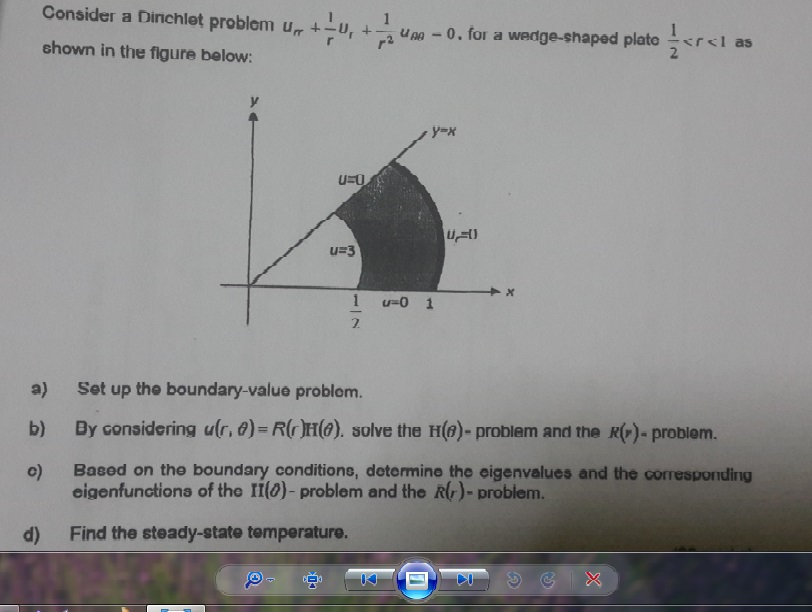
\includegraphics[width=0.6\textwidth]{wedge2.jpg}
%\caption{Steady-state temperature in a $45^\circ$ sector}
\end{figure}
\shabox{Solution}\\
a) BVP
\begin{align}
u_{rr}+\frac{1}{r}u_r+\frac{1}{r^2}u_{\theta\theta}&=0,\,\,\frac{1}{2}<r<1\label{w1}\\
s.t&\\
u(r,0)&=0,\,\,\frac{1}{2}<r<1\label{w2}\\
u(\frac{1}{2},\theta)&=3,\,\,0<\theta<\frac{\pi}{4}\label{w3}\\
u_r(1,\theta)&=0,\,\,0<\theta<\frac{\pi}{4}\label{w4}\\
u(r,\frac{\pi}{4})&=0,\,\,\frac{1}{2}<r<1\label{w5}
\end{align}
b) By considering $u(r,\theta)=R(r)H(\theta)$, solve the $H(\theta)$-problem and the $R(r)$-problem.\\
From \eqref{w1},
\begin{align}
R^{''}H+\frac{1}{r}R^{'}H+\frac{1}{r^2}RH^{''}&=0\nonumber\\
r^2R^{''}H+rR^{'}H+RH^{''}&=0\nonumber\\
r^2R^{''}H+rR^{'}H&=-RH^{''}\nonumber\\
\frac{r^2R^{''}+rR^{'}}{R}&=-\frac{H^{''}}{H}=\lambda\nonumber
\end{align}
leads to two ODEs
\begin{align}
r^2R^{''}+rR^{'}-\lambda R&=0\label{w1a}\\
H^{''}+\lambda H&=0\label{w1b}
\end{align}
We are looking for 
\begin{equation}
H^{''}+\lambda H=0,\,\label{w1aa}
\end{equation}
The three possibles general solution of \eqref{w1aa},
\begin{align}
H(\theta)&=c_1+c_2\theta,\,\,\lambda=0\label{w1ab}\\
H(\theta)&=c_1\,\cosh\,\alpha\theta+c_2\,\sinh\,\alpha\theta,\,\,\lambda=-\alpha^2<0\label{w1ac}\\
H(\theta)&=c_1\,\cos\,\alpha\theta+c_2\,\sin\,\alpha\theta,\,\,\lambda=\alpha^2>0\label{w1ad}
\end{align}
%Solution \eqref{w1ab} is nonperiodic unless we define $c_2=0$. 
The solution of Cauchy-Euler \eqref{w1a} are as follows. Let $R=r^m, R^{'}=mr^{m-1}, R^{''}=m(m-1)$. Substitute into \eqref{w1a} and for $\lambda=0$, becomes
\begin{align*}
r^2m(m-1)r^{m-2}+rmr^{m-1}&=0\\
m(m-1)r^m+mr^{m}&=\\
m^2r^m&=0\\
m&=0,0\leftarrow\shabox{equal real, $R(r)=c_1r^m+c_2r^m\,\ln\,r$}
\end{align*}
Thus the solution is
\begin{equation}
R(r)=c_1+c_2\,\ln\,r\label{swr1}
\end{equation}
For $\lambda_n=\alpha^2$, \eqref{w1a} becomes
\begin{align*}
r^2m(m-1)r^{m-2}+rmr^{m-1}&-\alpha^2 r^m=0\\
(m^2-\alpha^2)r^m&=0\\
m&=\alpha, -\alpha\leftarrow\shabox{real and different olution$R(r)=c_1r^{m_1}+c_2r^{-m_2}$}
\end{align*}
Thus the solution is
\begin{equation}
R(r)=c_1r^\alpha+c_2r^{-\alpha}\label{swr2}
\end{equation}
%--------------------
c) \underline{Apply BC on $H$-problem:}\\
\\
The BC \eqref{w2} and \eqref{w5}{w5} together with \eqref{w1a}  constitute a regular Sturm-Liouville problem\\


Now apply BC \eqref{w2} and \eqref{w5}: $u(r,0)=R(r)H(0)=0$. Since $R(r)\neq 0$, so $H(0)=0$. $u(r,\pi/4)=0\to H(\frac{\pi}{4})=0$.\\
The regular Sturm-Liouville problem:\\
\begin{equation}
H^{''}+\lambda H=0,\,\,H(0)=0,\,\,H(\frac{\pi}{4})=0.\label{sv1}
\end{equation}
From \eqref{w1ab} gives
\begin{align}
H(0)&=c_1+c_2(0)=0\to c_2=0\nonumber\\
So\,\,H(\theta)&=c_1\\
H(\frac{\pi}{4})&=c_1=0\to c_1=0
\end{align}
Thus $u(r,\theta)=0$ when $\lambda=0$.\\
From \eqref{w1ac},
\begin{align}
u(r,0)&=c_1\,\cosh(0)+c_1\,\sinh(0)=0\nonumber\\
&=c_1=0\to\,c_1=0.\nonumber\\
So\, u(r,\theta)&=c_2\,\sinh\,\alpha\theta\label{sw1}
\end{align}
From BC \eqref{w5}: $u(r,\frac{\pi}{4})=R(r)H(\frac{\pi}{4})=0\to H(\frac{\pi}{4})=0$. %Let $\lambda_n=\alpha^2=n^2$, $n=0, 1,2\ldots $, from \eqref{sw1},
\begin{align*}
u(r,\frac{\pi}{4})&=c_1\,\sinh\,\alpha\frac{\pi}{4}
\end{align*}
%For nontrivial solution $c_2\neq 0$, so $\sin\,\alpha\frac{\pi}{4}=0\to \alpha=4n$. So  the problem \eqref{sv1} possesses eigenvalues $\lambda_n=4n,\,\,n=1,2,\ldots$. The eigenfunction is
%\begin{equation}
%H(\theta)=c_2\,\sin\,4n\theta,\,\,\,n=1,2,3,\ldots\label{sow1}
%\end{equation}


%is nonperiodic and unbounded unless when $n=0$. So the solution is $u(r,\theta)=0$.\\
This solution is unbounded and nonperiodic unless $c_1=0$, So the solution is trivial.\\
Now apply BC \eqref{w2} and \eqref{w5} on \eqref{w1ad},
\begin{align*}
u(r,0)&=c_1\,\cos(0)+c_2\,\sin(0)=0\\
&=c_1=0\to c_1=0
\end{align*}
%----------------------
For nontrivial solution $c_2\neq 0$, so $\sin\,\alpha\frac{\pi}{4}=0\to \alpha=4n$. So  the problem \eqref{sv1} possesses eigenvalues $\lambda_n=4n,\,\,n=1,2,\ldots$. The eigenfunction is
\begin{equation}
H(\theta)=c_2\,\sin\,4n\theta,\,\,\,n=1,2,3,\ldots\label{sow1}
\end{equation}
%So the solution will be $2\pi$-periodic if we take $\alpha=n,\,\,n=1,2,\ldots$. Thus $u(r\,\theta)=c_1\,\sin\,n\theta$.\\
%Now use BC \eqref{w5} gives
%\begin{align*}
%u(r,\frac{\pi}{4})&=c_1\sin\,\frac{n\pi}{4}
%\end{align*}
\underline{Apply BC on $R$-problem}:\\
Transform  BC \eqref{w3} %and \eqref{w4} 
give $R^{'}(1)=0$. From \eqref{swr1}
\begin{align*}
R(r)&=c_1+c_2\,\ln\, r\\
R^{'}(r)&=\frac{c_2}{r}\\
R^{'}(0)&=\frac{c_2}{1}\to c_2=0
\end{align*}
$R(r)=C_1$,
So the solution is trivial.\\
Since we want $R(r)$ to be bounded as $r\to 0$, so eqn \eqref{swr2} we find that $c_2=0$ and $\lambda=\alpha=4n$. Thus \eqref{swr2} becomes
\begin{equation}
R(r)=c_1r^{4n}\label{sof1}
\end{equation}
%-------------------
d) From \eqref{sow1} and \eqref{sof1} we obtain a product solution
\begin{align*}
u_n(r,\theta)&=R(r)H(\theta)\\
&=c_1r^{4n}(c_2\,\sin\,4n\theta)\\
&=A_nr^{4n}\sin\,4n\theta
\end{align*}
And by using the superposition principle we obtain the solution of the steady-state temperature,
\begin{equation}
u(r,\theta)=\sum_{n=1}^\infty\,A_nr^{4n}\,\sin\,4n\theta\label{sowl}
\end{equation}
Now find $A_n$: apply BC $u(1/2,\theta)=3$
\begin{align*}
u(\frac{1}{2},\theta)=3&=\sum_{n=1}^\infty\,A_n\left(\frac{1}{2}\right)^{4n}\\
A_n\left(\frac{1}{2}\right)^{4n}&=\int_0^{\frac{\pi}{4}}3\,\sin\,4n\theta\,d\theta\\
&=\frac{3}{4n}[-\cos\,4n\theta]_0^{\frac{\pi}{4}}\\
&=\frac{3}{4n}(-\cos\,4n\frac{\pi}{4}+1)\\
&=\frac{3}{4n}(1-(-1)^n)\\
A_n&=\frac{3\cdot 2^{4n}}{4n}(1-(-1)^n)
\end{align*}
Therefore the steady-state temperature is
\begin{equation}
u(r,\theta)=\frac{3}{4}\sum_{n=1}^\infty\,\frac{(2r)^{4n}(1-(-1)^n)}{n}\,\sin\,4n\theta
\end{equation}
%----------------
\section{Domain of Disk, Semi-Disk, Annulus and Wedge}
\begin{enumerate}
\item The Dirichlet Problem:
\begin{figure}[hbt!]\centering
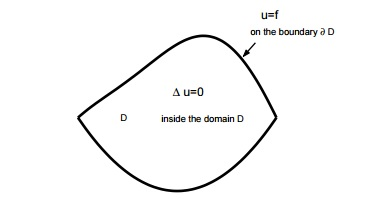
\includegraphics[width=0.6\textwidth]{domain1.jpg}
\caption{The Dirichlet Problem}
\end{figure}
%---------------------
\item The Neumann Problem:
\begin{figure}[hbt!]\centering
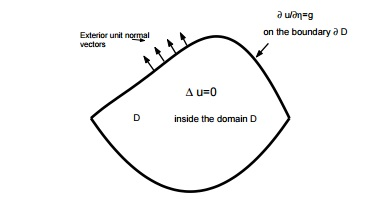
\includegraphics[width=0.6\textwidth]{domain2.jpg}
\caption{The Neumann Problem}
\end{figure}
\item Let a disk of radius, $r=a$. The domains are\\
A wedge: $0<r<a; 0 < \beta$;\\
An annulus: $0<a<r< b$;\\
Exterior of a circle: $a<r<b$:
\end{enumerate}
\section{Q5 Jan 2013}
\begin{description}
\item a) The solution Laplace equation in polar
$u_{rr}+\frac{1}{r}u_r+\frac{1}{r^2}u_{\theta\theta}=0$\\
is given as\\
$u(r,\theta)=A_0+B_0\,\ln\,r+ \sum_{n=1}^\infty\left(A_nr^{-n}+B_nr^n\right)\cos\,n\theta+\left(C_nr^{-n}+D_nr^n)\sin\,n\theta\right)$\\
State the domain that describe heat distribution in,
\begin{description}
\item i) Disk,
\item ii) Annulus,
\item iii) Exterior Domain.
\end{description}
\item b) Consider a semi circular disk of radius $r=1$. The temperature on its circumference is governed by the function,
$$f(\theta)=\pi\,\sin\,\theta-\sin\,2\theta $$
while on its diameter the temperature is zero.
\begin{description}
\item i) Express the problem as a boundary problem in polar variables.
\item ii) Let the solution be $u(r,\theta)=R(r)T(\theta)$ where $T(\theta)$ the angular component of the solution. By the separation of variables show that the solution, $u(r,\theta)$, within the semi circular disk is $u(r,\theta)=\pi r\,\sin\,\theta-r^2\sin\,2\theta$.
\end{description}
\end{description}
\shabox{Solution}\\
a) Let radius of the disk is $r=b$. The the domain of 
\begin{description}
\item Disk:$ D=\{0<r\le b,\,0<\theta\le 2\pi\}$
\item Annulus: $D=\{a<r<b,\,0<\theta\le 2\pi\}$ where $a$= inner circumference of the disk, $b$=outer circumference of the disk.
\item Exterior domain: $D=\{b<r<\infty,\,\,0\theta\le 2\pi\}$
\end{description}
b) i) BVP
\begin{align*}
u_{rr}+\frac{1}{r}u_r+\frac{1}{r^2}u_{\theta\theta}&=0,\,\,0<r\le r,\,\,0<\theta<\le \pi\\
s.t\hspace{2cm}&\\
u(r,0)&=0,\,\,0<r\le 1\\
u(r,\pi)&=0,\,\,0<r\le 1,\,\,0<\theta\le \pi\\
u(1,\theta)&=\pi\,\sin\,\theta-\sin\,2\theta,\,\,0<\theta\le\pi
\end{align*}
ii)\\
Using the separation variable method $u(r,\theta)=R(r)T(\theta)$ and distribute into PDE gives
\begin{align}
R^{''}T+\frac{1}{r}R^{'}T+\frac{1}{r^2}RT^{''}&=0\nonumber\\
r^2R^{''}T+rR^{'}T+RT^{''}&=0\nonumber\\
\frac{r^2R^{''}+rR^{'}}{R}&=-\frac{T^{''}}{T}=\lambda\nonumber
\end{align}
leads to two ODEs,
\begin{align}
r^2R^{''}+rR^{'}-\lambda R&=0\label{Q5j12a}\\
T^{''}+\lambda T&=0\label{Q5ja12b}
\end{align}
Translate BC : $u(r,0)=R(r)T(0)=0\to T(0)=0$, since $R(r)\neq 0$. And BC: $u(r,\pi)=R(r)T(\pi)=0\to T(\pi)=0$ since $R(r)\neq 0$.\\
ODE \eqref{Q5ja12b} together the translated BC above will constitute the Sturm-Liouville problem,
\begin{equation}
T^{''}+\lambda T=0,\,\,T(0)=0,\,\,T(\pi)=0\label{Q5j12c}
\end{equation}
The solution of \eqref{Q5j12c} are
\begin{align}
T(\theta)&=c_1+c_2\theta,\,\,\text{for}\,\lambda=0\label{soq5j12a}\\
T(\theta)&=c_1\,\cosh\,\alpha\theta=c_2\,\sinh\,\alpha\theta,\,\text{for}\,\lambda=-\alpha^2<0\label{soq5j12b}\\
T(\theta)&=c_1\,\cos\,\alpha\theta+c_2\,\sin\,\alpha\theta,\,\,\text{for}\,\,\lambda=\alpha^2>0\label{soq5j12c}
\end{align}
Now use BC: $T(0)=0$ and $T(\pi)=0$:
\begin{align*}
T(0)&=c_1+c_2(0)\to c_1=0\\
T(\theta)&=c_1\\
T(\pi)&=c_1=0\to c_1=0
\end{align*}
Thus $u(r,\theta)=0$, a trivial solution. \\
Eqn \eqref{soq5j12b},
\begin{align*}
T(0)&=c_1\,\cosh(0)=c_2\,\sinh(0)\to c_1=0\\
T(\theta)&=c_1\,\cosh\,\alpha\theta\\
T(\pi)&=c_1\cosh\,\alpha\phi=0\to c_1=0
\end{align*}
Thus the solution is trivial.\\
Next apply BC, $T(0)=0$ and $T(\pi)=0$ on \eqref{soq5j12c} gives
\begin{align*}
T(0)&=c_1\,\cos\,(0)+c_2\,\sin\,\alpha(0)\\
&=c_1(0)+0\to c_1=0\\
T(\theta)&=c_1\,\sin\,\alpha\theta\\
T(\pi)&=c_1\,\sin\,\alpha\pi=0
\end{align*}
For non trivial solution, $c_1\neq 0$, but $\sin\,\alpha\pi=0$. So $\alpha\pi=n\pi\to\alpha=n$. Thus the eigenvalue $\lambda_n=\alpha^2=n^2,\,\,n=1,2,\ldots$ and the correspondence eigen function of \eqref{Q5j12c} ,
\begin{equation}
T(\theta)=c_1\,\sin\,n\theta\label{sso1}
\end{equation}
Now we solve the Chauchy-Euler  problem \eqref{Q5j12a}. Let $R=r^m,\,R^{'}=mr^{m-1},\,R^{''}=m(m-1)r^{m-2} $ and substitute into \eqref{Q5j12a} becomes
\begin{align}
r^mm(m-1)t^{m-2}+rmr^{m-1}-\lambda r^m&=0\nonumber\\
(m^2-m+m)r^{m}&=0\leftarrow\shabox{for $\lambda_0=0$}\nonumber\\
m&=0,0\nonumber\\
\text{So}\,\,\,R(t)&=c_1+c_2\,\ln\,r\leftarrow\shabox{$R(r)=c_1\,r^m+c_2\,r^m\,\ln\,r$}\label{sso2}\\ 
r^mm(m-1)r^{m-2}+rmr^{m-1}-n^2r^m&=0\leftarrow\shabox{for $\lambda_n=\alpha^2$, $n=1,2,\ldots$}\nonumber\\
(m^2-n^2)r^m&=0\nonumber\\
m&=n,-n\nonumber\\
\text{So}\,\,R(t)&=c_1r^n+c_2r^{-n}\leftarrow\shabox{real and different roots}\label{sso3}
\end{align}
For periodic solution $c_2=0$ of \eqref{sso2} and for bounded solution $c_2=0$ of \eqref{sso3}. A product solution is 
\begin{equation}
u_n(r,\theta)=c_1r^n\,c_1\,\sin\,n\theta
\end{equation}
By superposition principle, the solution is
\begin{equation}
u(r,\theta)=\sum_{n=1}^\infty\,A_nr^n\,\sin\,n\theta\leftarrow\shabox{$A_n=c_1c_2$}
\end{equation}
Now apply BC: $u(1,\theta)=\pi\,\sin\,\theta-\sin\,2\theta$ becomes
\begin{align*}
u(1,\theta)=\pi\,\sin\,\theta-\sin\,2\theta &=\sum_0^\infty(\pi\,\sin\,\theta-\sin\,2\theta)A_n(1^n)\sin\,n\theta\,d\theta\\
A_n&=\frac{2}{\pi}\int_0^\pi(\pi\,\sin\,\theta-\sin\,2\theta)\sin\,n\theta\,d\theta\\
&\leftarrow\shabox{half range of $\pi\,\sin\,\theta-\sin\,2\theta$ in sine series}\\
&=\frac{2}{\pi}\int_0^\pi\,\pi\,\sin\,n\theta\,\sin\,\theta\,d\theta-\frac{2}{\pi}\int_0^\pi\,\sin\,2\theta\,\sin\,n\theta\,d\theta
\end{align*}
For different value of $n$ gives the results is zero (orthogonality).\\
Now For $n=1\to A_1$:
\begin{align*}
A_1&=\frac{2}{\pi}\int_0^\pi\,\pi\,\sin^2\theta\,d\theta\\
&=\frac{2}{\pi}\int_0^\pi\frac{\pi(1-\cos\,2\theta)}{2}\,d\theta\\
&=[\theta-\frac{1}{2}\sin\,2\theta]_0^\pi\\
&=(\pi-0)-0=\pi
\end{align*}
For $n=2\to A_2$;
\begin{align*}
A_2&==\frac{2}{\pi}\int_0^\pi\,\sin^2\,2\theta\,d\theta\\
&=\frac{2}{\pi}\int_0^\pi\left(\frac{1-\cos\,2\theta}{2}\right)d\theta\\
&=\frac{1}{\pi}[\theta-\frac{1}{2}\sin\,2\theta]_0^\pi\\
&=\frac{1}{\pi}((1-0)-0)\\
&=1
\end{align*}
The solution is
\begin{align*}
u(r,\theta)&=A_1r\,\sin\,n\theta+A_2r^n\,\sin\,n\theta\\
&=\pi\,r\,\sin\,\theta-r^2\,\sin\,2\theta
\end{align*}
\subsection{Graph of $u(r,\theta)=\pi\,r\,\sin\,\theta-r^2\,\sin\,2\theta$}
%%% Created by Maple 16.01 (IBM INTEL NT)
%% Source Worksheet: Untitled (1)
%% Generated: Fri Dec 04 14:55:04 2015
%\documentclass{article}
%\usepackage{maple2e}
 %\def\emptyline{\vspace{12pt}}
%\DefineParaStyle{Maple Output}
%\DefineParaStyle{Maple Plot}
%\DefineCharStyle{2D Math}
%\DefineCharStyle{2D Output}
%\begin{document}
%\pagestyle{empty}
\begin{maplegroup}
\begin{mapleinput}
\mapleinline{active}{1d}{restart;}{%
}
\end{mapleinput}

\end{maplegroup}
\begin{maplegroup}
\begin{mapleinput}
\mapleinline{active}{1d}{a:=Pi*r*sin(theta)-r^2*sin(2*theta);}{%
}
\end{mapleinput}

\mapleresult
\begin{maplelatex}
\mapleinline{inert}{2d}{a := Pi*r*sin(theta)-r^2*sin(2*theta);}{%
\[
a := \pi \,r\,\mathrm{sin}(\theta ) - r^{2}\,\mathrm{sin}(2\,
\theta )
\]
%
}
\end{maplelatex}

\end{maplegroup}
\begin{maplegroup}
\begin{mapleinput}
\mapleinline{active}{1d}{plot3d(a,r=0..1,theta=0..Pi,axes=boxed);}{%
}
\end{mapleinput}

\mapleresult
\begin{center}
\mapleplot{q5jan1201.eps}
\end{center}

\end{maplegroup}
\begin{maplegroup}
\begin{mapleinput}
\mapleinline{active}{1d}{?plot3d}{%
}
\end{mapleinput}

\end{maplegroup}
\begin{maplegroup}
\begin{mapleinput}
\end{mapleinput}

\end{maplegroup}
%\end{document}
%% End of Maple 16.01 Output

% dari maple
\begin{maplegroup}
\begin{mapleinput}
\mapleinline{active}{1d}{restart;}{%
}
\end{mapleinput}

\end{maplegroup}
\begin{maplegroup}
\begin{mapleinput}
\mapleinline{active}{1d}{a:=Pi*r*sin(theta)-r^2*sin(2*theta);}{%
}
\end{mapleinput}

\mapleresult
\begin{maplelatex}
\mapleinline{inert}{2d}{a := Pi*r*sin(theta)-r^2*sin(2*theta);}{%
\[
a := \pi \,r\,\mathrm{sin}(\theta ) - r^{2}\,\mathrm{sin}(2\,
\theta )
\]
%
}
\end{maplelatex}

\end{maplegroup}
\begin{maplegroup}
\begin{mapleinput}
\mapleinline{active}{1d}{plot3d(a,r=0..1,theta=0..Pi,axes=boxed);}{%
}
\end{mapleinput}

\mapleresult
\begin{center}
\mapleplot{q5jan1201.eps}
\end{center}

\end{maplegroup}
\begin{maplegroup}
\begin{mapleinput}
\mapleinline{active}{1d}{?plot3d}{%
}
\end{mapleinput}

\end{maplegroup}
\begin{maplegroup}
\begin{mapleinput}
\end{mapleinput}

\end{maplegroup}
%-------------------
\subsection{APR 2011}
\shabox{Q5}\\
\shabox{a)}\\
\underline{$H(\theta)$-problem}:Consider $u(r,theta)=R(r)H(\theta)$. Substitute into PDE give
\begin{align}
r^2R^{''}+rR^{'}-\lambda R&=0,\,\,a<r<b\label{q5ap11}\\
H^{''}+\lambda H&=,\,\,0\le\theta\le\pi\label{q5ap11a}
\end{align}
Eqn \eqref{q5ap11a} together with BC constitutes Sturm-Lioville problem
\begin{equation}
H^{''}+\lambda H=0,\,\,H(0)=0,\,\,H(\pi)=0\label{q5ap11b}
\end{equation}
Solve problem \eqref{q5ap11b} becomes
\begin{align}
H(\theta)&=c_1+c_2\theta\leftarrow\shabox{for $\lambda=0$}\label{q5ap11c}\\
H(\theta)&=c_1\,\cosh\,\alpha\theta+c_2\,\sinh\,\alpha\theta\leftarrow\shabox{for $\lambda=-\alpha^2<0$}\label{q5ap11d}\\
H(\theta)&=c_1\,\cos\,\alpha\theta+c_2\,\sin\,\alpha\theta\leftarrow\shabox{for $\lambda=\alpha^2>0$}\label{q5ap11e}
\end{align}
Apply BC:\\
For \eqref{q5ap11c},
\begin{align*}
H(0)=0=c_1+c_2(0)\to c_1=0\\
H(\theta)&=c_1\\
H(\pi)&=c_1=0\to c_1=0
\end{align*}
Thus \eqref{q5ap11c} gives  trivial solution.\\
For \eqref{q5ap11d},
\begin{align*}
H(0)&=c_1(1)+c_2(0)\to c_1=0\\
H(\theta)&=c_2\,\sinh\,\alpha\theta\\
H(\pi)&=c_1\,\cosh(\alpha\pi)=0\to c_1
\end{align*}
Similarly, \eqref{q5ap11d} gives trivial solution.\\
Now for \eqref{q5ap11e} gives
\begin{align*}
H(0)&=c_1(1)+c_2(0)\to c_1=0\\
H(\theta)&=c_2\,\sin\,\alpha\theta\\
H(\pi)&=c_2\,\sin\,\alpha\pi=0
\end{align*}
For non trivial solution, $c_2\neq 0$ but $\sin\,\alpha\pi=0\to \alpha\pi=n\pi\to\alpha=n$ That is $\lambda=n^2$.So the solution
\begin{equation}
H(\theta)=c_2\,\sin\,n\theta,\,\,n=1,2,\ldots\label{soq5ap11a}
\end{equation}
\underline{$R(r)$-Problem}:Now solve Chauchy-Euler \eqref{q5ap11}. Let $R=r^m$ gives
\begin{align*}
r^2m(m-1)r^{m-2}+rmr^{m-1}-\lambda r^m&=0\\
(m^2-\lambda)r^m&=0\\
m&=0,0\leftarrow\shabox{for $\lambda=0$ and}\\
(m^2-n)r^m&=0\\
m&=n,-n\leftarrow\shabox{for $\lambda=n^2$}
\end{align*}
gives the following results
\begin{align}
R(r)&=c_1+c_2\,\ln\,r\label{soq5ap11b}\\
R(r)&=c_1r^n+c_2r^{-n}\label{soq5ap11c}
\end{align}
For bounded to $r=0$, \eqref{soq5ap11b} and \eqref{soq5ap11c} becomes
\begin{align}
R(r)&=c_1\label{soq5ap11d}\\
%R(r)&=c_1r^n\label{soq5ap11e}
\end{align}
A product solution is
\begin{equation}
u_n(r,\theta)=(c_1r^n+c_2r^{-n})c_2\,\sin\,n\theta
\end{equation}
By superposition principle, the solution is
\begin{align}
u(r,\theta)&=\sum_{n=1}^\infty\,[(c_1r^n+c_2r^{-n})\,\sin\,n\theta\label{soq5ap11f}
%&=\sum_{n=1}^\infty\,A_nr^n\,\sin\,n\theta+B_nr^{-n}\sin\,n\theta]\leftarrow\shabox{$A_n=c_1c_2$ and $B_n=c_2c_2$}\label{soq5ap11f}
\end{align}
%-----------------
\shabox{c}\\
Now use BC: $(b,\theta)=0$:
From \eqref{soq5ap11c},
\begin{align*}
R(b)&=c_1b^n+c_2b^{-n}=0\to c_2=-c_1b^{2n}
\end{align*}
Substitute into \eqref{soq5ap11f}
\begin{align}
u(r,\theta)&=\sum_{n=1}^\infty\left(c_1r^n+c_2r^{-n}\right)c_2\,\sin\,n\theta\\
&=\sum_{n=1}^\infty c_1\left(r^n-\frac{b^{2n}}{r^n}\right)c_2\,\sin\,n\theta\\
&=\sum_{n=1}^\infty\,A_n\left(\frac{r^{2n}-b^{2n}}{r^n}\right)\sin\,n\theta\leftarrow\shabox{$A_n=c_1c_2$}\label{saa1}
\end{align}
%----------------
\shabox{d)}
\begin{align*}
A_n\left(\frac{a^{2n}-b^{2n}}{a^n}\right)&=\frac{2}{\pi}\int_0^\pi\,2\theta^2\,\sin\,n\theta\,d\theta\\
&=\frac{4}{\pi}\left[\theta^2\int\,\sin\,n\theta\,d\theta-\int[\int\,\sin\,n\theta\,d\theta\right]\frac{d}{\theta}(\theta^2)\,d\theta\\
&=\frac{4}{\pi}\left[\theta^2(-\frac{1}{n}\cos\,n\theta)+\frac{2}{n}\int\,\theta\,\cos\,n\theta\,d\theta\right]\\
&=-\frac{4}{n\pi}\theta^2\cos\,n\theta\big|_0^\pi+\frac{8}{n\pi}\left(\theta\,\int\,\cos\,n\theta\,d\theta-\int[\int\,\cos\,n\theta\,d\theta]d\theta\right)\\
&=-\frac{4\pi}{n}((-1)^n)+\frac{8}{n\pi}[\frac{\theta}{n}\,\sin\,n\theta\big|_0^\pi+\frac{1}{n^2}\cos\,n\theta\big|_0^\pi]\\
&=-\frac{4}{n\pi}((-1)^n)+\frac{8}{n^3\pi}((-1)^n-1)\\
&=\frac{(-8+8(-1)^n-4n^2\pi^2(-1)^n}{n^3\pi}\\
%&=\frac{(8-4n^2)}{n^3\pi}((-1)^n-1)\\
%A_n&=\frac{a^n(8-4n^2)}{n^3\pi(a^{2n}-b^{2n})}\left[(-1)^n-1\right]
A_n&=\frac{a^n(-8+8(-1)^n-4n^2\pi^2(-1)^n}{n^3\pi(a^{2n}-b^{2n}}
\end{align*}The solution is given by \eqref{saa1} where $A_n$ is the above eqn.
%----------------

%\chapter 7
\chapter{OCT 2010}
\section{Q5 QCT 2010}
\shabox{Q5 OCT 2010}
\begin{figure}[!ht]
\centering
 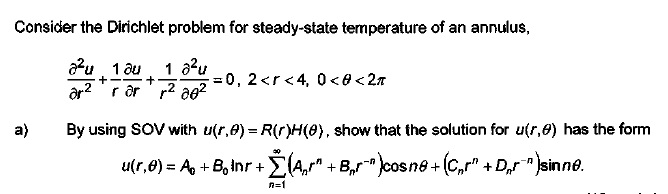
\includegraphics[width=0.8\textwidth]{q8oct10.jpg}    %insert your file at 'imagey1'
%\caption{$\mathbb{Z}_6$} \label{z6}
\end{figure}
\begin{figure}[!ht]
\centering
 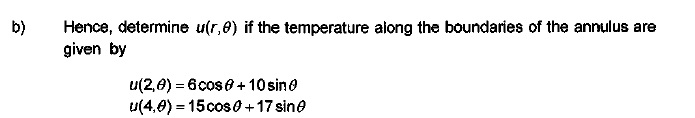
\includegraphics[width=0.8\textwidth]{q8oct10a.jpg}    %insert your file at 'imagey1'
%\caption{$\mathbb{Z}_6$} \label{z6}
\end{figure}\\
%----------------
\shabox{Solution}\\
a)
By using SOV $u(r,\theta)=R(r)H(\theta)$ and substitute into PDE gives two ODEs
\begin{align}
rR^{''}+rR^{'}-\lambda R&=0\label{q5oc10a}\\
H^{''}+\lambda H&=0\label{q5oc10b}
\end{align}
 We are seeking a solution of the \underline{$H(\theta)$-Problem }
 \begin{equation}
H^{''}+\lambda H=0,\,H(\theta)=H(\theta+2\pi)\label{q5oc11c}
\end{equation}
It will form an orthogonal set on the interval $[0,2\pi]$.\\
The three possible general solution s of \eqref{q5oc10b},
\begin{align}
H(\theta)&=c_1+c_2\theta,\,\,\lambda=0\label{q5oc11e}\\
H(\theta)&=c_1\,\cosh\,\alpha\theta+c_2\,\sinh\,\alpha\theta,\,\,\lambda=-\alpha^2<0\label{q5oc11f}\\
H(\theta)&=c_1\,\cos\,\alpha\theta+c_2\,\sin\,\alpha\theta,\,\,\,\lambda=\alpha^2>0\label{q5oc11g}
\end{align}
Solution \eqref{q5oc11e} is periodic if $C_2=0$. Similarly, solution \eqref{q5oc11f} is periodic if $c_1=c_2=0$.The constant solution
\begin{equation}
H(\theta)=c_1\label{soq5oc11a}
\end{equation}
can be assigned any period, and so $\lambda=0$ is an eigenvalue.\\
Solution \eqref{q5oc11g} will be $2\pi$-periodic if $\alpha=n$, where $n=1,2,\ldots$. \\The eigenvalues of \eqref{q5oc11g} are $\lambda_0=0$ and $\lambda_n=n^2,\,n=1,2,\ldots$.\\
The correspondence  eigenfunctions are
\begin{align}
H(\theta)&=c_1,\,n=0\label{soq5oc11a}\\
H(\theta)&=c_1\,\cos\,n\theta+c_2\,\sin\,n\theta,\,\,n=1,2,\ldots\label{soq5oc11c}
\end{align}
\underline{$R(r)$-Problem}:\\
The Chauchy-Euler DE \eqref{q5oc10a} are
\begin{align}
R(r)&=c_1+c_2\,\ln\,r,\,\,n=0\label{soq5oc11d}\\
R(r)&=c_1r^n+c_2r^{-n}\,\,n=1,2\ldots\label{soq5oc11e}
\end{align}
Thus product solution $u_n=R(r)H(\theta)$ for Laplace's equation  polar are
\begin{align*}
u_0&=(c_1+c_2\,\ln\,r)(c_1)\\
&=c_1c_1+c_1c_2\,\ln\,r\\
&=A_0+B_0\,\ln\,r\leftarrow\shabox{$A_0=c_1c_1$ and $B_0=c_1c_2$}\\
u_n&=(c_1r^n+c_2r^{-n})(c_1\,\cos\,n\theta+c_2\,\sin\,n\theta)\\
&=(c_1c_1r^n+c_1c_2r^{-n})\cos\,n\theta+(c_1c_2r^n+c_2c_2r^{-n})\sin\,n\theta\\
&=(A_nr^n+B_nr^{-n})\cos\,n\theta+(C_nr^n+D_nr^{-n})\sin\,n\theta
\end{align*}
The superposition principle then gives the solution
\begin{equation}
u(r,\theta)=A_0+B_0\,\ln\,r+\sum_{n=1}^\infty\,\left((A_nr^n+B_nr^{-n})\cos\,n\theta+(C_nr^n+D_nr^{-n})\sin\,n\theta\right)\label{soq5oc11f}
\end{equation}
b)\\
\underline{Apply BC: $u(2,\theta)=6\,cos\,\theta+ 10\,\sin\,\theta$}
\begin{align*}
u(2,\theta)=6\,\cos\,\theta+ 10\,\sin\,\theta&=A_0+B_0\ln\,2+\sum_{n=1}^\infty\,\left((A_n2^n+B_n2^{-n})\cos\,n\theta+(C_n2^n+D_n2^{-n})\sin\,n\theta\right)\\
%----------------
A_0+B_0\,\ln\,2&=\frac{1}{2\pi}\int_0^{2\pi}(6\,\cos\,\theta+ 10\,\sin\,\theta)d\theta\\
&=\frac{1}{2\pi}\left[6\,\sin\,\theta-10\,\cos\,\theta\right]_0^{2\pi}\\
&=\frac{1}{2\pi}(0-10(1-1))=0\\
%\text{So}\,\,\,\,A_0+B_0\,\ln\,r&=0
\end{align*}
%-------------------------
So
\begin{equation}
A_0+B_0\ln\,2=0\label{sor1}
\end{equation}
\begin{align}
u(2,\theta)=6\,\cos\,\theta+ 10\,\sin\,\theta&=\sum_{n=1}^\infty\,(A_n2^n+B_n2^{-n})\cos\,n\theta\\
A_n2^n+B_n2^{-n}&=\frac{1}{\pi}\int_0^{2\pi}(6\,\cos\,\theta+10\,\sin\,\theta)\cos\,n\theta\\
&=\frac{1}{\pi}\left(\int_0^{2\pi}\,6\,cos\,\theta\,\cos\,n\theta\,d\theta+\int_0^{2\pi}10\,\sin\,\theta\,\cos\,n\theta\right)\\
\text{when}\,\,n=1&\\
2A_1+\frac{B1}{2}&=\frac{1}{\pi}(6\pi)+0\\
&=6
\end{align}
Thus 
\begin{equation}
4A_1+B_1=12\label{sor2}
\end{equation}
\begin{align*}
C_n2^n+D_n2^{-n}&=\frac{1}{\pi}\int_0^{2\pi}[6\,\cos\,\theta+10\,\sin\,\theta]\sin\,n\theta\,d\theta\\
%\text{When $n$=1}&\\
2C_1+\frac{D_1}{2}&=\frac{1}{\pi}\int_0^{2\pi}6\,\cos\,\theta\,\sin\,\theta\,d\theta+\frac{1}{\pi}\int_0^{2\pi}\,10\,\sin\,\theta\,\sin\,\theta\,d\theta\\
&=\frac{1}{\pi}\sin^2\,\theta\big|_0^{2\pi}+\frac{10}{\pi}\int_0^{2\pi}\sin^2\,\theta\,d\theta\\
&=0+\frac{10}{\pi}\int_0^{2\pi}\frac{1-\cos\,2\theta}{2}\\
&=\frac{10}{\pi}\left[\frac{\theta}{2}-\frac{1}{4}\sin\,2\theta\right]_0^{2\pi}\\
&=10\\
\text{So}\,\,2C_1+\frac{D_1}{2}&=10
\end{align*}
Thus
\begin{equation}
4C_1+D_1=20\label{sorr1}
\end{equation}
\underline{Now apply BC: $u(4,\theta)=15\,\cos\,\theta+17\,\sin\,\theta$}:
\begin{align*}
A_0+B_0\, \ln\,4&=\frac{1}{2\pi}\int_0^{2\pi}(15\,\cos\,\theta+17\,\sin\,\theta)d\theta\\
&=0
\end{align*}
Thus
\begin{align}
A_0+B_0\ln\,4&=0\label{ssr1}
\end{align}
From \eqref{so1} and \eqref{ssr1} give $A_0=0,\,B_0=0$.\\
Next,
\begin{align*}
A_n4^n+B_n4^{-n}&=\frac{1}{\pi}\int_0^{2\pi}(15\,\cos\,\theta+17\,\sin\,\theta)\cos\,n\theta\,d\theta\\
4A_1+\frac{B_1}{4}&=\frac{1}{\pi}\int_0^{2\pi}(15\,\cos\,\theta\,\cos\,\theta+17\,\sin\,\theta\,\cos\,\theta)d\theta\leftarrow\shabox{Orthogonal series expansion: $n=1$}\\
&=\frac{1}{\pi}(15\pi+0)\\
&=15\\
\text{so},\,\,4A_1+\frac{B_1}{4}&=15
\end{align*}
Thus 
\begin{equation}
16A_1+B_1=60\label{ssr2}
\end{equation}
From \eqref{sor2} and \eqref{ssr2}; \eqref{ssr2}-\eqref{sor2} gives
\begin{align*}
12A_1&=48\\
A_1&=4\\
16(4)+B_1&=60\\
B_1&=-4
\end{align*}
Finally, 
\begin{align*}
C_n4^n+D_n4^{-n}&=\frac{1}{\pi}\int_0^{2\pi}(15\,\cos\,\theta+17\,\sin\,\theta)\sin\,n\theta\,d\theta\\
4C_1+\frac{D_1}{4}&=\frac{1}{\pi}\int_0^{2\pi}(15\,\cos\,\theta\,\sin\,\theta+17\,\sin\,\theta\,\sin\,\theta)d\theta\leftarrow\shabox{Orthogonal series expansion: $n=1$}\\
&=\frac{1}{\pi}(0+17\pi)\\
&=17\\
\text{so},\,\,4A_1+\frac{B_1}{4}&=17
\end{align*}
Thus 
\begin{equation}
16C_1+D_1=68\label{sorr2}
\end{equation}
Apply \eqref{sorr1} and \eqref{sorr2}, we solve for $C_1$ and $D_1$. \eqref{sorr2}-\eqref{sorr1} gives
\begin{align*}
12C_1&=48\\
C_1&=4\\
16(4)+D_1&=68\\
D_1&=4
\end{align*}
The solution is
\begin{equation}
u(r,\theta)=(4r-4r^{-1})\cos\,\theta+(4r+4r^{-1})\sin\,\theta
\end{equation}
\subsection{Q4 APR 2010}
\shabox{Q4}
\begin{figure}[!ht]
\centering
 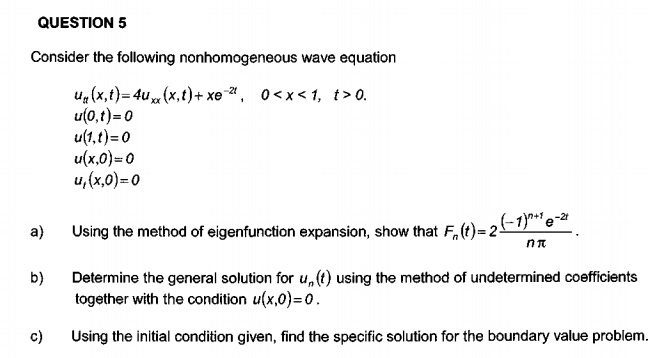
\includegraphics[width=\textwidth]{q5ap10.jpg}    %insert your file at 'imagey1'
%\caption{$\mathbb{Z}_6$} \label{z6}
\end{figure}\\
\shabox{Solution}\\
a)\\
The eigenvalues and eigenfunctions of 
\begin{equation}
%\end{}
X^{''}+\lambda X=0, X(0)=0,\,X(1)=0
\end{equation}
are found to be 
\begin{equation}
\lambda_n=\alpha_n^2=n^2\pi^2\,\,\text{and}\,\,\sin\,n\pi x,\,n=1,2,3,\ldots
\end{equation}
If we assume that
\begin{align}
u(x,t)&=\sum_{n=1}^\infty\,u_n(t)\,\sin\,n\pi x\nonumber\\
u_{xx}&=\sum_{n=1}^\infty\,u_n(t)(-n^2\pi^2)\,\sin\,n\pi x\label{q4ap10a}\\
u_{tt}&=\sum_{n=1}^\infty\,u_n^{''}(t)\,\sin\,n\pi x\label{q4ap10b}
\end{align}
We can write $F(x,t)=xe^{-2t}$
\begin{align}
xe^{-2t}&=\sum_{n=1}^\infty\,F_n(t)\,\sin\,n\pi x\nonumber\\
F_n(t)&=\frac{2}{1}\int_0^1\,xe^{-2t}\sin\,n\pi x\,dx\\
&=2e^{-2t}\int_0^1\,x\,\sin\,n\pi x\,dx\nonumber\\
&=2e^{-2t}\left[\frac{-x}{n\pi}\cos\,n\pi x+\frac{1}{n\pi}\int\,\cos\,n\pi x\,dx\right]\nonumber\\
&=2e^{-2t}\left[-\frac{x}{n\pi}\,\cos\,n\pi x+\frac{1}{n^2\pi^2}\sin\,n\pi x\right]_0^1\\
&=2e^{-2t}\left(\frac{-1}{n\pi}(-1)^n\right)\nonumber\\
&=2e^{-2t}\left(\frac{1}{n\pi}(-1)^{n+1}\right)\nonumber\\
xe^{-2t}&=\sum_{n=1}^\infty\left(2e^{-2t}\left(\frac{1}{n\pi}(-1)^{n+1}\right)\right)\sin\,n\pi x\label{q4ap10c}
\end{align}
%------------------
So $F_n(t)=2\left(\frac{(-1)^{n+1}}{n\pi}\right)e^{-2t}$


b) Substitute \eqref{q4ap10a}, \eqref{q4ap10b} and \eqref{q4ap10c} into PDE gives
\begin{align}
u_{tt}-4u_{xx}&=xe^{-2t}\\
\sum_{n=1}^\infty\,\left[u_n^{''}(t)+4n^2\pi^2u_n(t)\right]\sin\,n\pi x&=\sum_{n=1}^\infty\left(2e^{-2t}\left(\frac{1}{n\pi}(-1)^{n+1}\right)\right)\sin\,n\pi x\label{q4ap10d}
\end{align}
By equating the coefficients of $\sin\,n\pi x$,
\begin{align}
u_n^{''}(t)+4n^2\pi^2u_n(t)&=2e^{-2t}\left(\frac{1}{n\pi}(-1)^{n+1}\right)\label{q4ap10e}
%u_n^{''}&=\frac{(-1)^{n+1}}{n\pi}2e^{-2t}-4n^2\pi^2u_n(t)\\
%u_n^{'}&=
\end{align}
Solve \eqref{q4ap10e} by using undetermined coefficients;
Auxiliary equation
\begin{align*}
m^2+4n^2\pi^2&=0\\
m&=2n\pi i,\,-2n\pi i\leftarrow\shabox{complex roots}
\end{align*}
The complementary solution,
\begin{equation}
u_{nc}(t)=c_1\,\cos\,2n\pi t+c_2\,\sin\,2n\pi t\label{a4ap10f}
\end{equation}
Particular solution 
\begin{align*}
u_{np}(t)&=Be^{-2t}\\
u^{'}&=-2Be^{-2t}\\
u^{''}&=4Be^{-2t}\\
%&=4(Bx+c)e^{-2t}-4Be^{-2t}
\end{align*}
Substitute into \eqref{q4ap10e} gives
\begin{align*}
4Be^{-2t}+4n^2\pi^2Be^{-2t}&=\left(\frac{2(-1)^{n+1}}{n\pi}\right)\\
%(4C-4B+4n^2\pi^2C)e^{-2t}+(4B+4n^2\pi^2)xe^{-2t}&=\left(\frac{(-1)^{n+1}}{n\pi}\right)2e^{-2t}\\
\end{align*}
By equating the coefficient of  and $e^{-2t}$ becomes
\begin{align}
B(4+4n^2\pi^2)&=\left(\frac{2(-1)^{n+1}}{n\pi}\right)
%B+2n^2\pi^2&=\left(\frac{(-1)^{n+1}}{n\pi}\right)\label{sso1}\\
\label{sso2}
\end{align}
From \eqref{sso2} gives
\begin{equation}
B=\frac{(-1)^{n+1}}{2n\pi(1+n^2\pi^2)}\label{sso3} 
\end{equation}

%subtitute \eqref{sso3} into \eqref{sso1}
%\begin{align*}
%4C+4n^2\pi^2+2n^2\pi^2&=\left(\frac{(-1)^{n+1}}{n\pi}\right)\\
%4C&=\left(\frac{(-1)^{n+1}}{6n^3\pi^3}\right)\\
%C&=\left(\frac{(-1)^{n+1}}{24n^3\pi^3}\right)\\
%u_p(t)&=
%\end{align*}
Thus the particular solution
\begin{equation}
u_{np}(t)=\left(\frac{(-1)^{n+1}}{2n\pi(1+n^2\pi^2)}\right)e^{-2t}
\end{equation}
Hence the general solution
\begin{align*}
u_n(t)&=u_{nc}+u_{np}\\
&=c_1\,\cos\,2n\pi t+c_2\,\sin\,2n\pi t+\left(\frac{(-1)^{n+1}}{2n\pi(1+n^2\pi^2)}\right)e^{-2t}
\end{align*}
Apply $u(x,0)=0$:
\begin{align*}
u_n(x,0)=0&=c_1(1)+0+\frac{(-1)^{n+1}}{2n\pi(1+n^2\pi^2)}\\
c_1&=\frac{(-1)^{n+2}}{2n\pi(1+n^2\pi^2)}
\end{align*}
Hence the general solution
\begin{align}
u_n(t)&=\left(\frac{(-1)^{n+2}}{2n\pi(1+n^2\pi^2)}\right)\cos\,2n\pi t+c_2\,\sin\,2n\pi t+\left(\frac{(-1)^{n+1}}{2n\pi(1+n^2\pi^2)}\right)e^{-2t}
\end{align}
%--------------------
c) 
The solution,

\begin{align}
u(x,t)&=\sum_{n=1}^\infty\left[\left(\frac{(-1)^{n+2}}{2n\pi(1+n^2\pi^2)}\right)\cos\,2n\pi t+c_2\,\sin\,2n\pi t+\left(\frac{(-1)^{n+1}}{2n\pi(1+n^2\pi^2)}\right)e^{-2t}\right]\sin\,n\pi x\label{sss1}
\end{align}
Apply BC: $u_t(x,0)=0$:
\begin{align}
u_t(x,t)&=\sum_{n=1}^\infty\left[\left(2\frac{(-1)^{n+2}}{2n\pi(1+n^2\pi^2)}\right)(-\sin\,2n\pi t)+2c_2\,\cos\,2n\pi t-2\left(\frac{(-1)^{n+1}}{2n\pi(1+n^2\pi^2)}\right)e^{-2t}\right]\sin\,n\pi x\nonumber\\
0&=2c_2-2\left(\frac{(-1)^{n+1}}{2n\pi(1+n^2\pi^2)}\right)\nonumber\\
c_2&=\left(\frac{(-1)^{n+1}}{2n\pi(1+n^2\pi^2)}\right)\label{ssss1}
\end{align}
Hence the solution VBP is given by \eqref{sss1} where $c_2$ is given by \eqref{ssss1}.


% chapter 8
\chapter{Jun 2014}
\shabox{Q5}\\
Given 
\begin{align*}
u_{rr}+\frac{1}{r}u-r+\frac{1}{r^2}u-{\theta\theta}&=0,\,r>c,\,\,-\pi\le\theta\le\pi\\
u(c,\theta)&=f(\theta),\,-\pi\le\theta\le\pi
\end{align*}
a) Determine the solutions for $R(r)$-problem:\\
Let $R=r^m,\,R^{'}=mr^{m-1},\,R^{''}=m(m-1)r^{m-2}$ and sunstitute into
\begin{align}
r^2R^{''}+rR^{'}-\lambda R&=0\\
r^2m(m-1)r^{m-2}+rmr^{m-1}-\lambda r^m&=0\\
(m^2-\lambda)r^m&=0\\
\text{Since $r^m\neq 0$},&\\
m&=0,0\leftarrow\shabox{for $\lambda=0$}\\
m&=n,-n\leftarrow\shabox{for $\lambda=n^2$}
\end{align}
The solution are
\begin{align}
R(r)&=c_1+c_2\,\ln\,r\label{q5j14a}\\
R(r)&=c_1r^n+c_2r^{-n}\label{q5j14b}
\end{align}
$R(r)$ are unbounded as $r$ approaches to $\infty$.\\
The solution of $R(r)$-problem are
\begin{align}
R(r)&=c_1\\
R(r)&=c_2r^{-n}
\end{align}


b)Thus The product  solution is
\begin{align}
u_n(r,\theta)&=A_0c_1+c_2r^{-n}(c_1\,\cos\,n\theta+c_2\,\sin\,n\theta)\\
&=B_0+r^{-n}(A_n\,\cos\,n\theta+B_n\,\sin\,n\theta)\leftarrow\shabox{$B_0=A_0c_1$, $A_n=c_1c_2$, $B_n=c_1c_2$}
\end{align}
Hence the general solution is
\begin{align}
u(r,\theta)&=B_0+\sum_{n=1}^\infty\,r^{-n}(A_n\,\cos\,n\theta+B_n\,\sin\,n\theta)\label{soq5j14}
\end{align}
Now apply BC:$f(\theta)=u(1,\theta)=\pi-|\theta|$
\begin{align*}
B_0&=\frac{1}{2\pi}\int_{-\pi}^{\pi}(\pi-|\theta|)\,d\theta\\
&=\frac{1}{2\pi}\int_{-\pi}^0(\pi-(-\theta))\,d\theta+\frac{1}{2\pi}\int_{0}^{\pi}(\pi-\theta)\,d\theta\\
&=\frac{1}{2\pi}\left[\pi\theta+\frac{1}{2}\theta^2\right]_{-\pi}^0+\frac{1}{2\pi}\left[\pi\theta-\frac{1}{2}\theta^2\right]_0^\pi\\
&=\frac{1}{2\pi}(0-(\pi^2+\frac{1}{2}\pi^2)+\frac{1}{2\pi}(\pi^2-\frac{1}{2}\pi^2)\\
&=\frac{1}{2}\pi
\end{align*}
\begin{align*}
A_n&=\frac{1}{\pi}\int_{-\pi}^\pi(\pi-|\theta|)\,\cos\,n\theta\,d\theta\\
&=\frac{1}{\pi}\int_{-\pi}^0(\pi+\theta)\cos\,n\theta\,d\theta+\frac{1}{\pi}\int_0^\pi(\pi-\theta)\cos\,n\pi\,d\theta\\
&=-\frac{(-1+(-1)^2)}{\pi n^2}+-\frac{(-1+(-1)^2)}{\pi n^2}\\
&=-\frac{2(-1+(-1)^n)}{\pi n^2}
\end{align*}
\begin{align}
B_n&=\frac{1}{\pi}\int_{-\pi}^\pi(\pi-|\theta|)\,\sin\,n\theta\,d\theta\nonumber\\
&=\frac{1}{\pi}\int_{-\pi}^0(\pi+\theta)\sin\,n\theta\,d\theta+\frac{1}{\pi}\int_0^\pi(\pi-\theta)\sin\,n\theta\,d\theta\nonumber\\
&=\frac{(-\pi n+\sin(\pi n))}{\pi n^2}-\frac{(-\pi n+\sin(\pi n))}{\pi n^2}\\
&=0
\end{align}
The solution is give by \eqref{soq5j14} where $B_0$, $A_n$ and $B_n$ is given by the above .




%\chap 7
\section{Dec 2013}
\shabox{Q5}\\
a) Apply SOV $u(x,y)=X(x)Y(y)$ gives two ODEs
\begin{align}
X^{''}+\lambda X&=0\label{q5de13a}\\
Y^{''}-\lambda Y&=0\label{q5de13b}
\end{align}
The Sturm-Liouville associated eqn \eqref{q5de13a} and BC then 
\begin{equation}
X^{''}+\lambda X=0,\,,X(0)=0,X(\pi)=0
\end{equation}
The solutions are
\begin{align}
X(x)&=c_1+c_2 x\leftarrow\shabox{$\lambda=0$}\label{q5de13c}\\
X(x)&=c_3\,\cosh\,\alpha x+c_4\,\sinh\,\alpha x\leftarrow\shabox{$\lambda=-\alpha^2<0$}\label{q5de13aa}\\
X(x)&=c_5\,\cos\,\alpha x+c_6\,\sin\,\alpha x\leftarrow\shabox{$\lambda=\alpha^2>0$}\label{q5dec13ab}
\end{align}

\begin{align*}
X(0)=0&=c_1+C_2(0)\to c_1\\
X(x)&=c_2x\\
X(\pi)=0&=c_2(\pi)\to c_2=0
\end{align*}
Thus The solution is trivial. Similarly for eqn \eqref{q5de13aa}.
For eqn \eqref{q5dec13ab}
\begin{align}
X(0)=0=c_5\,(1)+c_6(0)\to c_5=0\\
X(x)&=c_6\,\sin\,\alpha x\\
X(\pi)&=c_6\,\sin\,\alpha \pi
\end{align}
For non trivial solution $C_6\neq 0$ but $\sin\,\alpha \pi=0$ that is $\alpha\pi=n\pi\to \alpha=n$. Thus the solution is
\begin{equation}
X(x)=c_6\,\sin\,n x
\end{equation}
From ODE \eqref{q5de13b} with BC $u(x,1)=0\to Y(1)=0$
                                       
\bibliographystyle{mn}
\bibliography{cuba}
\printindex
\end{document}